%===============================================================================
% OBDH laboratory manual
%
% © 2020 Juan A. de la Puente <juan.de.la.puente@upm.es>
% © 2022 Juan Zamorano <juanrafael.zamorano@upm.es>
%
% Some rights reserved. This work is licensed under a  
% Creative Commons Attribution-NonCommercial-ShareAlike 4.0 International License.
% http://creativecommons.org/licenses/by-nc-sa/4.0/
%===============================================================================
\documentclass[12pt,a4paper,english,twoside]{book}

\bibliographystyle{abbrvnat}
\usepackage{natbib}

\usepackage[utf8]{inputenc}    % UTF8 encoding
%\usepackage{t1enc}                % Latin1 characters
%\usepackage{babel}                % hyphenation etc. - not needed 
\usepackage{graphicx}             % figures
\DeclareGraphicsExtensions{.pdf,.png,.jpg}
\graphicspath{{fig/}}
\usepackage{xcolor}

\usepackage{amssymb,amsmath}
\usepackage{alltt}
\usepackage[hmargin=3cm,vmargin=2cm]{geometry} % page margins
\usepackage{calc}
%\usepackage[lineno5]{lgrind}
\usepackage{hyperref}
%\usepackage{fontspec,xunicode,xltxtra}
\usepackage{gensymb}
\usepackage{float}
\usepackage{theorem}
\usepackage{listings}

\definecolor{mGreen}{rgb}{0,0.6,0}
\definecolor{mGray}{rgb}{0.5,0.5,0.5}
\definecolor{mPurple}{rgb}{0.58,0,0.82}
%\definecolor{mPurple}{rgb}{101, 41, 128}
\definecolor{backgroundColour}{rgb}{255,255,255}
% \definecolor{orangered}{RGB}{239,134,64}

%\lstset{inputpath=code/}
%\lstdefinestyle{CStyle}{
%    backgroundcolor=\color{backgroundColour},
%    commentstyle=\color{mGreen},
%    keywordstyle=\color{magenta},
%    numberstyle=\tiny\color{mGray},
%    stringstyle=\color{mPurple},
%    basicstyle=\footnotesize,
%    breakatwhitespace=false,
%    breaklines=true,
%    captionpos=b,
%    keepspaces=true,
%    numbers=left,
%    numbersep=5pt,
%    showspaces=false,
%    showstringspaces=false,
%    showtabs=false,
%    tabsize=4,
%    morekeywords={vTaskNotifyGiveFromISR},
%    language=C
%}

%\lstdefinestyle{c}{
%       language=c,
%       basicstyle=\sffamily,
%       xleftmargin=\parindent,
%       numbers=none,
%       columns=flexible,
%}

%------------- software versions ------------------------------------

%\newcommand{\simplicitystudio}{Simplicity
%Studio\textsuperscript{\tiny\texttrademark} 4 }
%\newcommand{\sdk}{Flex Software Development Kit (SDK) Gecko v5.0.0}
%\newcommand{\matlabversion}{Matlab R2018b}
%\newcommand{\gccversion}{\prog{GCC~7.2.1}}
%\newcommand{\gdbversion}{\prog{GDB~8.0}}
%\newcommand{\binutils}{\prog{binutils 2.29.51}}
%\newcommand{\newlibversion}{\prog{Newlib~2.5.0}}

%-------------- other commands ---------------------------------------
\newcommand{\prog}[1]{\textsf{#1}}

\newcommand{\program}[1]{{\ttfamily\upshape #1}}
\newcommand{\variable}[1]{{\slshape #1}}

%\newcommand{\prog}[1]{\texttt{#1}}

\theoremstyle{break}\newtheorem{warning}{WARNING}[chapter]

\newenvironment{entry}[1]
   {\begin{list}{}%
          {\renewcommand{\makelabel}[1]{\textbf{##1}\hfil}%
           \settowidth{\labelwidth}{\textbf{#1}}%
           \setlength{\leftmargin}{\labelwidth+\labelsep}%
          }%
   }%
   {\end{list}}

%\renewcommand{\CMfont}{\ttfamily\slshape}
%\renewcommand{\KWfont}{\ttfamily\bfseries}
%\renewcommand{\VRfont}{\ttfamily\upshape}
%\renewcommand{\BGfont}{\ttfamily\upshape}

%\renewcommand{\LGnuminterval}{1}

%======================= document ===================================
\begin{document}
%======================= front matter ===============================
\frontmatter

\begin{titlepage}

\begin{center}

\framebox{
\begin{minipage}{100mm}
\begin{center}
\textbf{STRAST/UPM}
\end{center}

This report describes the second laboratory assignment of Data Handling course.
\end{minipage}
}
\end{center}

\vfill\vspace{50pt}

\begin{center}
%\rule{\textwidth}{1pt}\\[2\baselineskip]
\textbf{\huge Data Handling}\\[\baselineskip]
{\large Máster Universitario en Sistemas Espaciales}\\[\baselineskip]
\textbf{\Huge Native and Cross-Development Environment Work}\\[\baselineskip]
{\large Version 1.0 --- \today}\\[\baselineskip]
{\large\textsc{2nd student assignment}}
\end{center}

\vfill

\begin{center}\textsc{
\rule{\textwidth}{1pt}\\
Universidad Politécnica de Madrid\\
Grupo STARST\\
Sistemas de Tiempo Real y Arquitectura de Sistemas Telemáticos\\}
\url{https://www.dit.upm.es/str}\\[1em]
\rule{\textwidth}{1pt}\\
\end{center}

\end{titlepage}

\thispagestyle{empty}


{\footnotesize
\noindent
\copyright\ 2021 STRAST/UPM.

\vspace{\baselineskip}\noindent
Published by
\begin{quote}
Grupo STRAST\\
Sistemas de Tiempo Real y Arquitectura de Sistemas Telem�ticos\\
%\url{https://www.dit.upm.es/str}\\
Universidad Polit�cnica de Madrid\\
Madrid\\
SPAIN
\end{quote}

\vspace{\baselineskip}\noindent
Permission is granted to make and distribute verbatim copies of this
manual provided the copyright notice and this permission notice are
preserved on all copies.

Permission is granted to copy and distribute modified versions of this
manual under the conditions for verbatim copying, provided also that
the sections entitled  Copying  and  GNU General Public License  (see
appendix \ref{ap:licence}) are included exactly as in the
original, and provided that the entire resulting derived work is
distributed under the terms of a permission notice identical to this
one.

Permission is granted to copy and distribute translations of this
manual into another language, under the above conditions for modified
versions, except that this permission notice may be stated in a
translation approved by the Free Software Foundation.

\vspace{\baselineskip}
\noindent
\begin{tabular}{lp{120mm}}
\textbf{Status:}  & Ongoing\\
\\
\textbf{Authors:}    & Juan Antonio de la Puente\\
                     & Juan Zamorano\\
\\
\textbf{Revised by:} & Juan Zamorano\\
\end{tabular}

\vspace{2\baselineskip}
\noindent
\begin{tabular}{llp{120mm}}
\textbf{History}\\
\textbf{Version}&\textbf{Date}&\textbf{Comments}\\
\end{tabular}

}







\cleardoublepage\pagestyle{plain}
%\pagenumbering{roman}
\setcounter{page}{1}
\setcounter{tocdepth}{1}
\tableofcontents

%======================= document body =================================
\mainmatter
\cleardoublepage
\pagestyle{headings}
\pagenumbering{arabic}\setcounter{page}{1}
%----------------------------------------------------------------------
%!TEX root = manual.tex
%===============================================================================
\chapter*{Introduction}\label{ch:introduction}
\addcontentsline{toc}{chapter}{Introduction}
%----------------------------------------------------------------------

This document provides instructions for laboratory work in the field of embedded systems. The laboratory is part of the Data Handling course of the UPM Máster Universitario de Sistemas Espaciales (MUSE) program.
The laboratory is based on a computer kit that is used to build a simplified version of a satellite on-board software system (OBSW). An instance of the laboratory kit will be made available to every student registered in the course during the laboratory session.

Students are required to use their own personal computer, running Windows, MacOS, or GNU/Linux, to carry out the laboratory assignments. 
The outline of the laboratory assignments to be carried out is as follows:
\begin{enumerate}
\item	Installation of a native programming environment.
\item	Installation of the cross-platform programming tools.
\item   Simple housekeeping program.
\item   Tasking program.
\item   Distributed program.
\item   Real-time program, including temporal analysis
\item	   Real-time program with Attitude Control System.
\item   On-board data handling (OBDH) system.
\end{enumerate}

%----------------------------------------------------------------------
\section*{References}
\addcontentsline{toc}{section}{References}

The following documents contain additional information about the software
and hardware tools used to develop the work:

\subsection*{Hardware}
\begin{enumerate}
\item	\href{https://www.st.com/resource/en/data\_brief/stm32f4discovery.pdf}{STMicroelectronics. DB1421 Data Brief.  STM32F4DISCOVERY - Discovery kit with STM32F407VG MCU.}
\item \href{https://www.st.com/content/ccc/resource/technical/document/user\_manual/70/fe/4a/3f/e7/e1/4f/7d/DM00039084.pdf/files/DM00039084.pdf/jcr:content/translations/en.DM00039084.pdf}{STMicroelectronics. UM1472 User manual - Discovery kit with STM32F407VG MCU.}
\item \href{https://www.st.com/resource/en/datasheet/dm00037051.pdf}{STMicroelectronics. DS 8626. Data sheet - STM32F405xx, STM32F407xx. ARM Cortex-M4 32b MCU+FPU, 210DMIPS, up to 1MB Flash/192+4KB RAM, USB OTG HS/FS, Ethernet, 17 TIMs, 3 ADCs, 15 comm. interfaces \& camera.}
\item \href{https://www.st.com/content/ccc/resource/technical/document/reference\_manual/3d/6d/5a/66/b4/99/40/d4/DM00031020.pdf/files/DM00031020.pdf/jcr:content/translations/en.DM00031020.pdf}{STMicroelectronics. RM0090 Reference manual - STM32F405/415, STM32F407/417, STM32F427/437 and STM32F429/439 advanced Arm\copyright-based 32-bit MCUs.}
\end{enumerate}

\subsection*{Software}

The following manuals are available from the ``Help" menu in the GNAT Programming Studio (GPS):
\begin{enumerate}
\item \href{http://www.ada-auth.org/standards/rm12i\_w\_tc1/html/RM-TTL.html}{Ada Reference Manual.}
\item	GPS User's Guide.
\item	GNAT User's Guide for Native Platforms.
\item	GNAT User's Guide Supplement for Cross Platforms
\item	GNAT Reference Manual.
\end{enumerate}

%----------------------------------------------------------------------

\section*{Acronyms}
\addcontentsline{toc}{section}{Acronyms}

\begin{entry}{RAVENSCAR}
\item[ADC] Analog to Digital Converter.
\item[ATC] Attitude Control System
\item[DAC] Digital to Analog Converter.
\item[FPU] Floating Point Unit.
\item[GCC] GNU compilation system..
\item[GDB] GNU Debugger.
\item[GNAT] GNU Ada TranslatorDebugger.
\item[GNU] GNU is not Unix.
\item[GPL] GNU Public License.
\item[GPS] GNAT Programming Studio.
\item[LGPL] Lesser GNU Public License (formerly Library GPL).
\item[MCU] Microcontroller Unit.
\item[OBC] On-Board Computer.
\item[OBDH] On-Board Data Handling.
\item[OBSW] On-Board Software.
\item[OS] Operating System.
\item[PC] IBM Personal Computer architecture.
\item[TC] Telecommand.
\item[TM] Telemetry.
\item[USART] Universal Synchronous Asynchronous Receiver Transmitter.
\item[USB] Universal Serial Bus.
\end{entry}


%----------------------------------------------------------------------
\chapter*{Overview}\label{ch:overview}
\addcontentsline{toc}{chapter}{Overview}
%----------------------------------------------------------------------

\section*{Laboratory kit components}
\addcontentsline{toc}{section}{Laboratory kit components}

The laboratory kit includes:
\begin{itemize}
\item	An STM32F407 computer board, which emulates an on-board computer system (OBC).
\item	A USB A / mini USB cable which is used to connect the OBC board to the development station hosted on the student PC.
\item	A USB / UART interface cable which is used to provide a serial line link between the OBC board and the ground station software running on the student PC.
\end{itemize}

Figure~\ref{fig:kit} shows the components of the laboratory kit and the connections to the student PC.

\begin{figure}[h]
            \centering{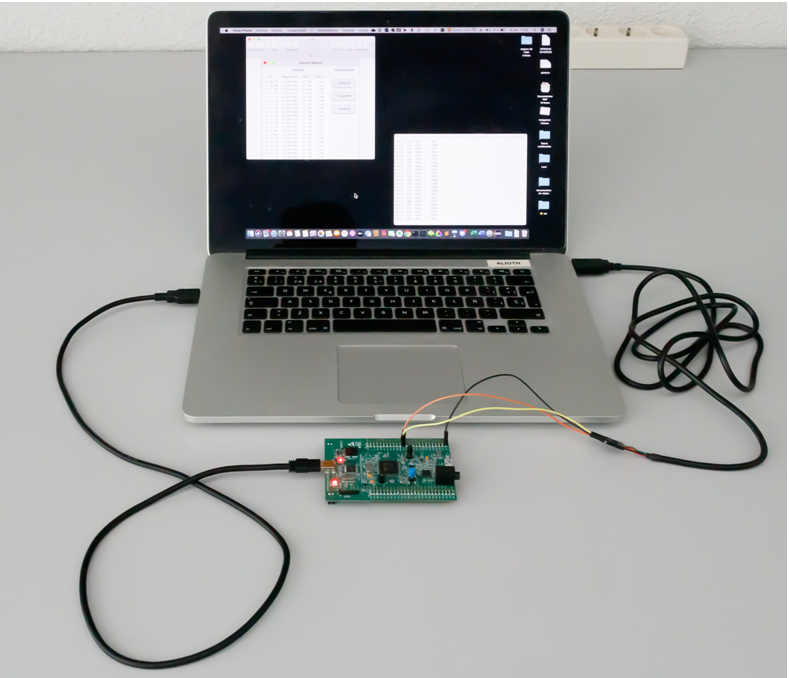
\includegraphics[width=.6\textwidth,keepaspectratio]{laboratory_kit.png}}
            \caption{Laboratory kit.}
            \label{fig:kit}
\end{figure}

\section*{Architecture of the laboratory platform}
\addcontentsline{toc}{section}{Architecture of the laboratory platform}

The components of the laboratory kit are used to emulate a simplified version of a satellite on-board software system. Figure~\ref{fig:architecture} shows the architecture of the laboratory system.

\begin{figure}[h]
            \centering{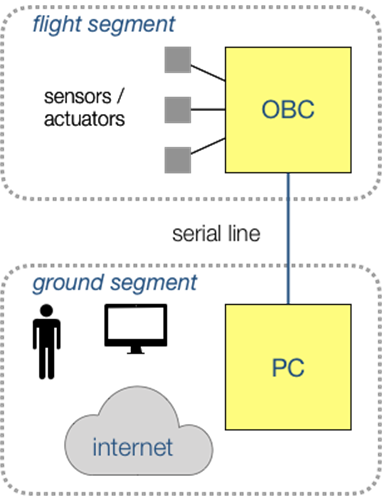
\includegraphics[width=0.35\textwidth,keepaspectratio]{architecture.png}}
            \caption{Architecture of the laboratory system.}
            \label{fig:architecture}
\end{figure}

The system consists of a flight segment, implemented on the laboratory computer board, and a ground system, implemented on the student PC. The communication between both segments is carried out by means of a serial line, simulating the radio link of a real satellite mission.
The student work is centered on programming the computer board. The ground station software will be provided by the teachers.

\section*{Computer board and connections}
\addcontentsline{toc}{section}{Computer board and connections}

The STM32F407 board is used as a low-cost replacement for a satellite on-board computer (OBC). The board features a 32-bit ARM Cortex-M4 microcomputer, 192 KB RAM, 1 MB Flash memory and a number of other devices.

Figure~\ref{fig:board} shows an overall view of the computer board.

\begin{figure}[h]
            \centering{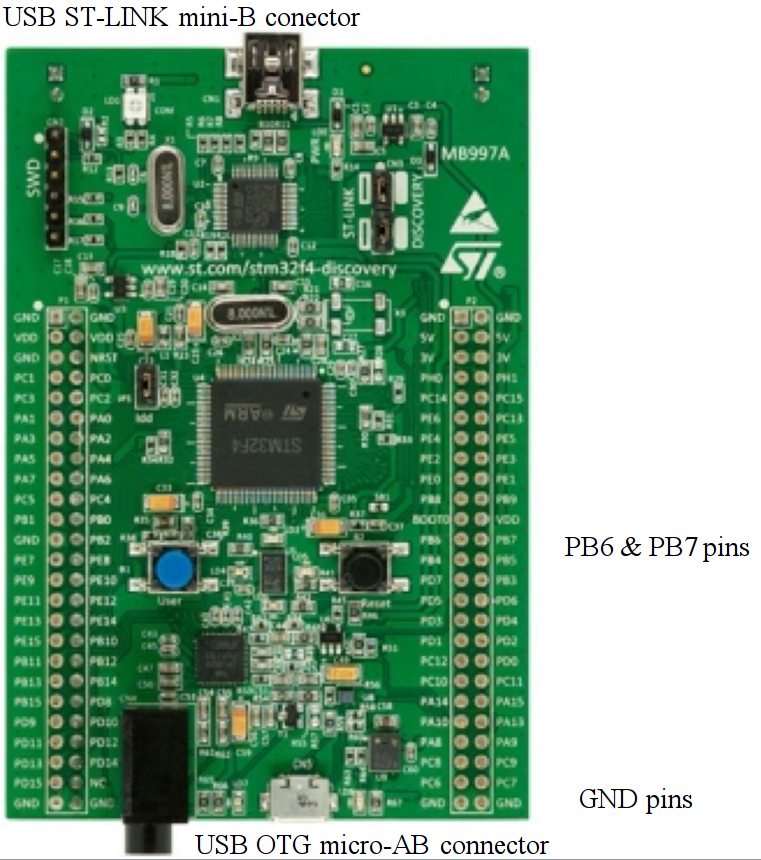
\includegraphics[height=11cm,keepaspectratio]{board.png}}
            \caption{Computer board.}
            \label{fig:board}
\end{figure}

The main elements that will be used in the laboratory are:
\begin{itemize}
\item	USB ST-LINK connector, which is linked to a PC with a mini USB-USB A cable. This connection is used for the following functions:
\begin{itemize}
\item	power supply to the board (5 V)
\item	program loading and debugging from host
\end{itemize}
\item	GPIO pins PB6, PB7 and GND. GPIO (General Purpose Input-Output) is a standard interface for connecting external devices. These GPIO pins are used in the laboratory to connect a serial line to a USB port on a PC, emulating the connection to the on-board radio equipment in a satellite.
\item	Temperature and voltage sensors. These sensors are part of the STM32 microcomputer chip, and can be read using internal registers in the MCU. They are used in the laboratory to emulate the housekeeping 
\end{itemize}

\renewcommand{\chaptername}{Assignment}
%!TEX root = manual.tex
%===============================================================================
\chapter{Install a native programming environment}\label{ch:Assignment1}

The aim of this assignment is to install a native programming environment for the Ada language on the student PC. This environment will later be extended with cross-compilation tools for the STM32 board to be used in the laboratory. 

The programming environment to be used is GNAT Community, an open-source software development environment freely available from AdaCore, a company specialised in providing tools and solutions for developing high-integrity software,
\section{Download and install GNAT}
The GNAT Community compilation system can be downloaded from \url{https://www.adacore.com/download/more}. Installation packages for Windows, MacOS and GNU Linux are available at the download page. The file {\tt README.txt} provides installation instructions, which are summarised as follows:
\subsection{Windows}
\begin{enumerate}
\item Download the file {\tt gnat-2021-20210519-x86\_64-windows64-bin.exe}
\item Run the file and follow the instructions.
\end{enumerate}
\subsection{MacOS}
\begin{enumerate}
\item Download the file {\tt gnat-2020-20200818-x86\_64-darwin-bin.dmg}
\item Open the dmg disk and execute the application inside it. In order to circumvent the system protection, control-click on the file and then click on ``opens" in the emergent window.
\end{enumerate}
Notice that you need to have installed the Xcode application to install GNAT. If you still see the following error:
\begin{verbatim}
ld: library not found for -lSystem
\end{verbatim}
then you might have to execute the following:
\begin{verbatim}
xcode-select -s /Applications/Xcode.app/Contents/Developer
\end{verbatim}
\subsection{GNU Linux}
\begin{enumerate}
\item Download the file {\tt gnat-2021-20210519-x86\_64-linux-bin}
\item You will need to make the package executable before running it. In a command prompt, execute the following command:
\begin{verbatim}
     chmod +x path\_to\_the\_package.bin
\end{verbatim}
and execute the package. The {\tt README.txt} file contains additional installation and execution instructions.
\end{enumerate}

\section{Test the installation with a simple program}

The GNAT compilation system includes the GPS (GNAT programming studio) programming environment, which allows users to edit, compile, and run Ada and C programs. Figure\ref{fig:gps} shows the main GPS window, which is composed of the following areas:

\begin{figure}[h]
            \centering{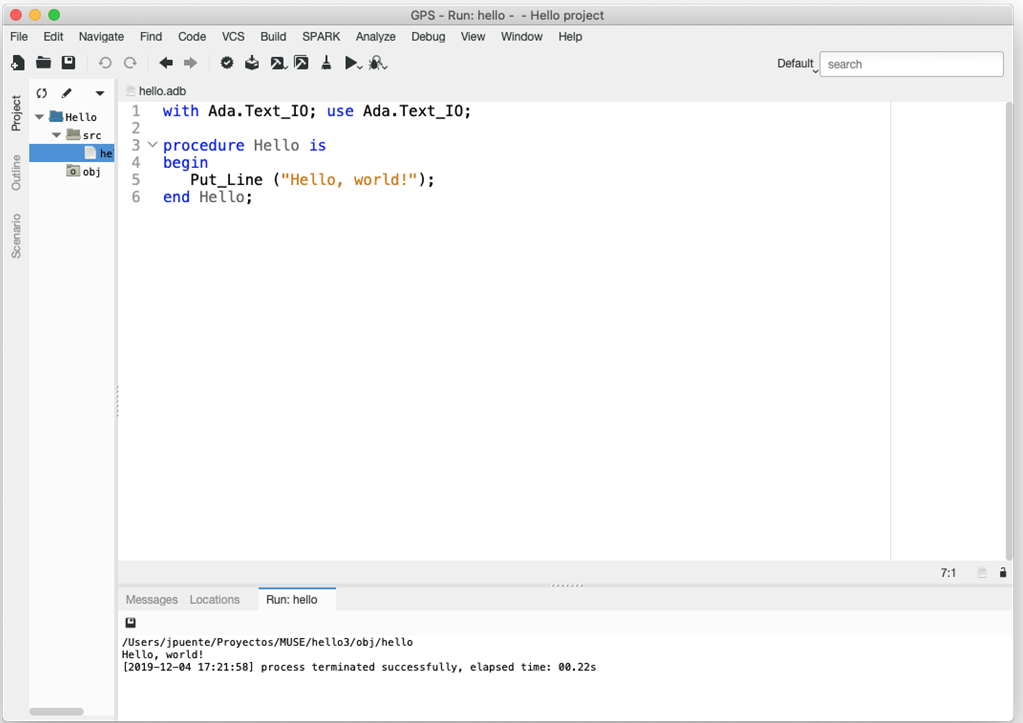
\includegraphics[width=\textwidth,keepaspectratio]{gps.png}}
            \caption{GNAT Programming Studio (GPS).}
            \label{fig:gps}
\end{figure}

\begin{itemize}
\item	a menu bar at the top
\item	a tool bar under the menu bar
\item	on the left, a notebook allowing you to switch between Project, Outline and Scenario views
\item	the working area in the center
\item	the messages window at the bottom
\end{itemize}

GPS organises source code in projects. A project is a set of source files which are compiled together in order to produce a single binary executable. 
Before starting you will need to create a folder to store your software projects. The recommendation is to create a folder named OBDH\_LABS in a directory of your choice.
The next activity is to write and run a simple Ada program using GPS:
\begin{enumerate}
\item 	Create a new project by clicking on {\tt File} > {\tt New Project} ... in the top menu. Choose the {\tt Simple Ada Project} template.
\item	Choose a folder to deploy the project, e.g. OBDH\_LABS/LAB1. Set the project name to {\tt Hello} and the main name also to {\tt Hello}.
\item	Double click on the {\tt hello.adb} file in the project view to open the file in the working area. 
\item	Edit the file in the working area so that it has the same content as in figure\ref{fig:gps}.
\item	Build and run the executable by clicking on the $\rhd$ symbol in the tool bar. You should see a number of compilation-related messages and, if everything is right, you will see the text ``Hello, world!" in the Run tab of the bottom window.
\end{enumerate}
%\begin{figure}[h]
%            \centering{\includegraphics[width=\textwidth,keepaspectratio]{gpshello.png}}
%            \caption{Hello world demo program.}
%            \label{fig:gpshello}
%\end{figure}



\chapter{Install the cross-compilation tools}\label{ch:Assignment2}

The aim is to get acquainted with the embedded computer board and to install and test the cross-compilation tools for GNAT that will be used to develop executable code for it.

\section{Cross-compilation tools}

The computer board will programmed in Ada. The GNAT cross-platform software development system will be used (figure~\ref{fig:cross}), where the student PC is the host platform and the SMT32 board is the target platform.

\begin{figure}[h]
            \centering{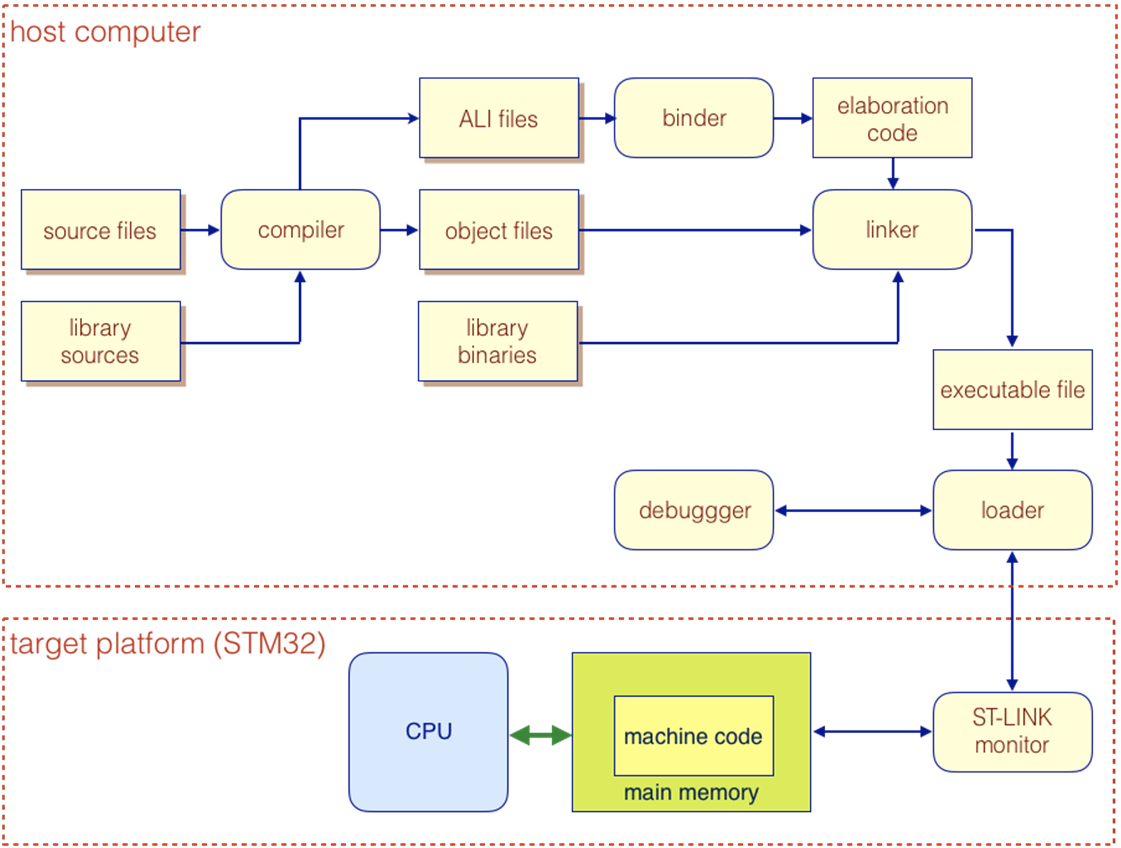
\includegraphics[width=\textwidth,keepaspectratio]{cross.png}}
            \caption{Cross-compilation and debugging system}
            \label{fig:cross}
\end{figure}

In order to compile a program, the compilation chain is run on the host computer to produce an executable file for the target computer. The executable is then loaded into the target memory, from where it can be run. A monitor program is preinstalled on the target board that supports loading and debugging from the host platform.

\section{Download and install GNAT ARM ELF}

GNAT ARM ELF is the cross-compilation chain to be used with the STM32F4 board. It can be downloaded from the same page as the native GNAT system, https://www.adacore.com/download/more, and there are installation packages for Windows, MacOS and GNU Linux available. The file {\tt README.txt} provides installation instructions, which are summarised as follows.
\subsection{Windows}
\begin{enumerate}
\item Select ARM ELF (hosted on windows64) and download the file\\
{\tt gnat-2021-20210519-arm-elf-windows64-bin.exe}
\item Run the file and follow the instructions.
\item You will also need to install the USB driver for the ST-LINK probe. To do so, go to \url{http://www.st.com/content/st\_com/en/products/embedded-software/development-tool-software/stsw-link009.html}, and click on {\tt Get Software}. Click on {\tt Get Software} under the {\tt Download} column of the table that shows up to obtain the driver. You will need to accept ST Micro's license agreement and enter your contact details. 
Once downloaded unzip the USB device driver and run the installer, accepting all the defaults.
\end{enumerate}
\subsection{MacOS}
\begin{enumerate}
\item Download the file {\tt gnat-community-2019-20190517-arm-elf-darwin-bin.dmg}
\item Open the dmg disk and execute the application inside it. In order to circumvent the system protection, control-click on the file and then click on ``open" in the emergent window.
\item You will also need the st-util,  st-flash, and st-info tools. You can download the binaries from 
\url{https://github.com/texane/stlink/releases/download/1.3.0/stlink-1.3.0-macosx-amd64.zip}. Unzip and copy the files in the bin directory to a directory in your {\tt PATH}. You may need to circumvent MacOS protection by executing the command:
\begin{verbatim}
	\$ xattr -d com.apple.quarantine path-to-executable-file
\end{verbatim}
\end{enumerate}
\subsection{GNU Linux}
\begin{enumerate}
\item Download the file {\tt gnat-2021-20210519-arm-elf-linux64-bin}
\item You will need to make the package executable before running it. In a command prompt, execute the following command:
\begin{verbatim}
     chmod +x path\_to\_the\_package.bin
\end{verbatim}
and then execute the package.
\item You will also need to install the stlink tools. In Ubuntu and Debian stlink must be installed from sources. Follow the instructions on \url{http://docs.adacore.com/live/wave/gnat\_ugx/html/gnat\_ugx/gnat\_ugx/arm-elf\_topics\_and\_tutorial.html\#linux}.
\end{enumerate}

The {\tt README.txt} file contains additional installation and execution instructions.

\section{Test your installation with an embedded program}

The next thing is to compile a run a simple embedded program. This program is only intended to test that the compilation chain and the ST-LINK tools have been properly installed.

Open GPS and do the following:
\begin{enumerate}
\item Create a new project by clicking on {\tt File} > {\tt New Project} ... in the top menu. Choose the {\tt STM324F compatible} > {\tt LED demo project template}.
\item	Choose a folder to deploy the project, e.g. OBDH\_LABS/LAB2. Set the project name to {\tt led\_demo} and the main name to {\tt main.} A window with a project including a number of source files will open.
\item	Right-click on the project icon on the left side area, and choose {\tt Project} > {\tt Properties} (figure 6). On the emerging window, select Embedded and change the Connection tool selector to st-util. Save the settings.
\item	Connect the STM32F4 board to the computer by means of a USB A / mini USB cable.
\item	Build the executable and load it into the board by clicking on the
\hbox{
\includegraphics[width=1.5em]{buildandload.png}} symbol in the tool bar (or select {\tt Build} > {\tt Bareboard} > {\tt Flash to board} on the top menu). You should see a number of compilation-related messages ending with ``Flashing complete. You may need to reset or cycle power".
\item	If everything is all right, you will see the LEDS on the board blinking in a circular pattern.
\item Download and install the Ada Drivers Library
The Ada Drivers Library is a set of Ada packages that make it easier to write software for embedded devices, including the STM32F4 microcontroller family and some demonstration boards. The source code can be found at \url{https://github.com/AdaCore/Ada\_Drivers\_Library}. To install the library, click on the green {\tt Clone} or {\tt download} button on the upper right side and then on Download Zip in the emerging window. You will get a zip archive in your downloads folder. Unzip the archive and move the resulting folder to your OBDH\_LABS folder. Rename the folder to {\tt Ada\_Drivers\_Library}, removing any trailing text.
\item Compile and run a test program with the Ada Drivers Library
\end{enumerate}
Open GPS and do the following:
\begin{enumerate}
\item Select {\tt Open} project on the welcome window. Navigate to .../OBDH\_LABS/\-Ada\_Drivers\_Library/examples/STMF4\_DISCO and open the project file: {\tt blinky\-\_f4disco.gpr}.
\item	Build the executable and load it into the board by clicking on the \hbox{
\includegraphics[width=1.5em]{buildandload.png}} symbol in the tool bar (or select {\tt Build} > {\tt Bareboard} > {\tt Flash to board} on the top menu). When the loading is complete, you will see the board LEDS blinking all at the same time.
\end{enumerate}

\section{Install MATLAB\texttrademark and Simulink\texttrademark}

MATLAB and Simulink will be used to generate C code from a Simulink model and 
to validate the system by Processor In the Loop (PIL).

UPM has a campus license available for students. \url{http://www.upm.es/sfs/Rectorado/Vicerrectorado\%20de\%20Tecnologias\%20de\%20la\%20Informacion\%20y\%20Servicios\%20en\%20Red/Servicio\%20de\%20Planificacion\%20Informatica\%20y\%20Comunicaciones/SW/MATLAB_UPM_Estudiantes.pdf} explains how to install MATLAB and Simulink.

In order to generate C code, the Embedded Coder toolbox and its dependencies must be installed.

%!TEX root = manual.tex
%===============================================================================
\chapter{Simple housekeeping program}\label{ch:Assignment3}

The aim of this assignment is to experiment with a simple housekeeping program that only implements a basic function, reading a temperature sensor on the on-board computer. The value read by the sensor is denoted as OBC\_T (OBC temperature).
The software is organised in modules, in such a way that it can be later extended to a more complex housekeeping system in the next assignments.

\section{Temperature sensor}

The internal temperature sensor in the MCU is used in this assignment. No additional hardware is required.

The STM32F407 reference manual (section 13.10) states that the internal temperature sensor of the MCU is internally cabled to the {\tt ADC1\_IN16} analog input channel. The steps required to read the sensor are:

\begin{enumerate}
\item Select {\tt ADC1\_IN16} input channel in the ADC.
\item Select a sampling time greater than the minimum sampling time specified in the datasheet (see table~\ref{tb:sensor} below).
\item Set the {\tt TSVREFE} bit in the {\tt ADC\_CCR} register to wake up the temperature sensor from power down mode.
\item Start the ADC conversion by setting the {\tt SWSTART} bit (or by external trigger).
\item Read the resulting VSENSE data in the ADC data register.
\item Calculate the temperature using the following formula:

Temperature (in \degree{C}) = {(VSENSE - V25) / Avg\_Slope} + 25

Where:
\begin{itemize}
\item V25 = VSENSE value for 25 \degree{C} (table~\ref{tb:sensor})
\item Avg\_Slope = average slope of the temperature vs. VSENSE curve (table~\ref{tb:sensor}).
\end{itemize}
\end{enumerate}

The sensor has a startup time after waking from power down mode before it can output VSENSE at the correct level. The ADC also has a startup time after power-on, so to minimize the delay, the {\tt ADON} and {\tt TSVREFE} bits should be set at the same time.

The sensor has a range of -40 to 125 \degree{C}, with a precision of $\pm$1.5 \degree{C}. Its main characteristics are described in the STM32F407 datasheet (table~\ref{tb:sensor}).

\begin{table}[htb]
\begin{center}
\begin{tabular}{llllll} \hline
Symbol & Parameter & Min & Typ & Max & Unit \\ \hline
TL & VSENSE linearity with temperature & - & $\pm1$ & $\pm2$ & \degree{C}\\
Avg\_Slope & Average slope & - & 2.5 & & mV/\degree{C}\\
V25 & Voltage at 25 \degree{C} & - & 0.76 & & V\\
tSTART & Startup time & - & 6 & 10 & $\mu{s}$\\
TS\_temp & ADC sampling time when reading & 10 & - & - & $\mu{s}$\\
& the temperature (1 \degree{C} accuracy) &  &  &  & \\ \hline
\end{tabular}
\caption{STM32F407 temperature sensor characteristic.}
\label{tb:sensor}
\end{center}
\end{table}

The Ada Drivers Library includes the package STM32.ADC, which provides facilities for handling the analog to digital converter.

\section{Software architecture}
The software architecture of the simple housekeeping program is depicted in figure~\ref{fig:simple}\footnote{The graphic notation is AADL (Architecture Analysis and Design Language).}. The software components are:

\begin{figure}[h]
            \centering{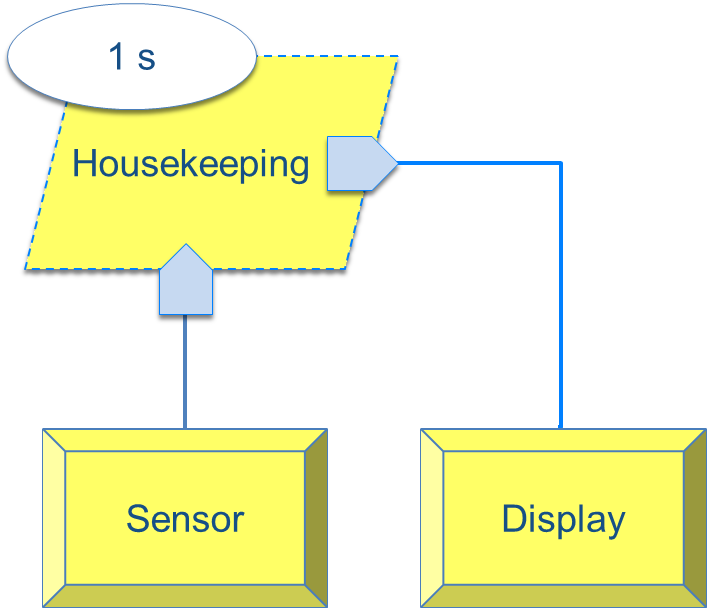
\includegraphics[width=0.5\textwidth,keepaspectratio]{simple.png}}
            \caption{Software architecture of simple housekeeping system.}
            \label{fig:simple}
\end{figure}

\begin{description}
\item[Housekeeping.] Main component, which performs the basic functionality of the system, i.e. reading a temperature value and displaying the value on the console.
\item[Sensor.] This module provides a high-level interface to the temperature sensor and deals with all the details of reading the ADC to which the sensor is connected.
\item[Display.] This module provides a high-level interface to a text console where the measured temperature values can be output.
\end{description}

Since the OBC board does not have a text output device, it has to be simulated on the host computer, using a mechanism called semihosting. When the target board is connected to the host by means of the ST-LINK USB cable, and the embedded program is run using the debugger in the host, the standard output is re-directed to the debugger console. The GPS environment supports semihosting.

\subsection{Download the code and study the implementation}

The implementation code, as initially provided to the students, can be downloaded from \url{https://github.com/STR-UPM/OBDH_LABS}. Click on {\tt Clone} or {\tt download}, download a zip archive, unzip and move to your work directory. The code for this assignment is in the LAB3 folder.

The {\tt Housekeeping} package is the root element of the housekeeping subsystem. Its specification consists of one procedure, {\tt Initialize}, that starts the operation of the component. It has three subpackages:

\begin{description}
\item[Housekeeping.Data] contains the definitions of the data types used in the subsystem. Only one data type, {\tt Analog\_Data}, is defined for this version of the software.

\item[Housekeeping.Sensor] contains the details of the temperature sensor. Its specification includes the {\tt Initialize} and {\tt Get} procedures. This package uses the Ada Drivers Library to interact with the OBC board hardware.

\item[Housekeeping.Display] includes the procedure {\tt Put}, which is used to display temperature values on the debugger console (see below). The original implementation of this procedure writes raw sensor values, which are integers in the range 0 to 4095, as directly provided by the ADC hardware. These values have to be converted to engineering units. i.e. degrees Celsius, using the steps shown in section 3.1 above. The software provided to the students includes a program, {\tt adc2celsius}, which implements this functionality.
\end{description}

The {\tt Display.Put} procedure uses the {\tt Ada.Text\_IO} package to write to the standard output.  Since there is no device that can be used to provide text output on the OBC board, the ST-LINK prove provides a facility, which is called semihosting, to provide this functionality. When the program is run using the cross-debugger on the host, the board standard output is redirected to the debugger console. Therefore, in order to see the temperature values the program must be run from the debugger (see below).

The main procedure is {\tt OBSW}\footnote{On-Board Software}. It calls {\tt Housekeeping.Initialize}, which initializes the sensor and then calls the {\tt Run} procedure. This procedure executes an endless loop that performs the following actions:
\begin{itemize}
\item Get a raw temperature measurement from the sensor
\item Display the value
\end{itemize}

Additionally, one of the board LEDs is toggled on and off to provide a visual check that the program is running.
Notice that {\tt Run}, and hence {\tt Initialize} and {\tt OBSW}, never return. Therefore the program executes indefinitely, as is common in embedded systems.

\section{Compile and run with the debugger.}

Open GPS and do the following:
\begin{enumerate}
\item Select {\tt Open project} on the welcome window. Navigate to the LAB3 directory and open the {\tt simple\_housekeeping.gpr} project file.
\item Build the executable and load it into the board by clicking on the \hbox{
\includegraphics[width=1.5em]{debug.png}} symbol in the tool bar (or select {\tt Build} $\rightarrow$ {\tt Bareboard} $\rightarrow$ {\tt Debug} on board on the top menu).

The program will be compiled, and the executable will be loaded into the board memory by the debugger. After that, the debugger is started\footnote{On Windows a message will be displayed requesting permission to connect st-util to external networks. Be sure to grant such permission to enable the debugger connection to the board.}, and the debugger console (lowest window in GPS) shows the following lines:
\begin{verbatim}
...
(gdb) monitor reset halt
(gdb)
\end{verbatim}

\item Type {\tt continue} or just {\tt c} on the debugger console (or select {\tt Debug} $\rightarrow$ {\tt Continue} on the top menu).
\begin{verbatim}
(gdb) c
Continuing.
[program running]
\end{verbatim}

\item The program will start running (check the LED blinking), and the raw temperature readings are shown on the {\tt Messages} tab of the debugger console (figure~\ref{fig:gdb-output}).
\end{enumerate}

\begin{figure}[h]
            \centering{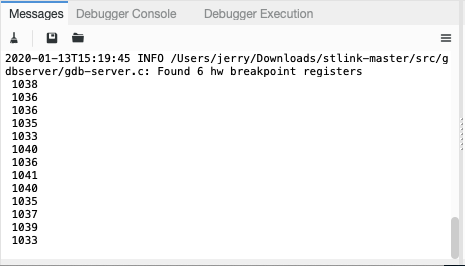
\includegraphics[width=0.8\textwidth,keepaspectratio]{gdb-output.png}}
            \caption{Debugger output.}
            \label{fig:gdb-output}
\end{figure}

The raw measurement values can be converted to Celsius using the {\tt adc2celsius} program. You should take into account that the internal temperature sensor does not provide an accurate measurement, and may have an offset that varies from one chip to another.

\section{Make changes to the program}

As a final activity, you may make some changes to the provided program in order to make sure that you understand the logics behind the source code. Proposed changes are:

\begin{enumerate}
\item Include the conversion to Celsius in the {\tt Display.Put} procedure.
\item Add the following statement to the main loop in the Housekeeping Run procedure:

{\tt delay until Clock + Milliseconds (1000);}

The effect of this statement is to delay the execution of the program for 1 s. You will have to import the {\tt Ada.Real\_Time} library package in order to use the operations included in the statement.
\end{enumerate}

\chapter{Tasking housekeeping program}\label{ch:Assignment4}

The aim of this assignment is to extend the simple housekeeping program of the previous assignment by adding a communications subsystem. The extended system includes two concurrent tasks communicating through a protected shared object.

\section{Software architecture}

The software architecture of the tasking housekeeping program is depicted in figure~\ref{fig:tasking}. The software components are:

\begin{figure}[h]
            \centering{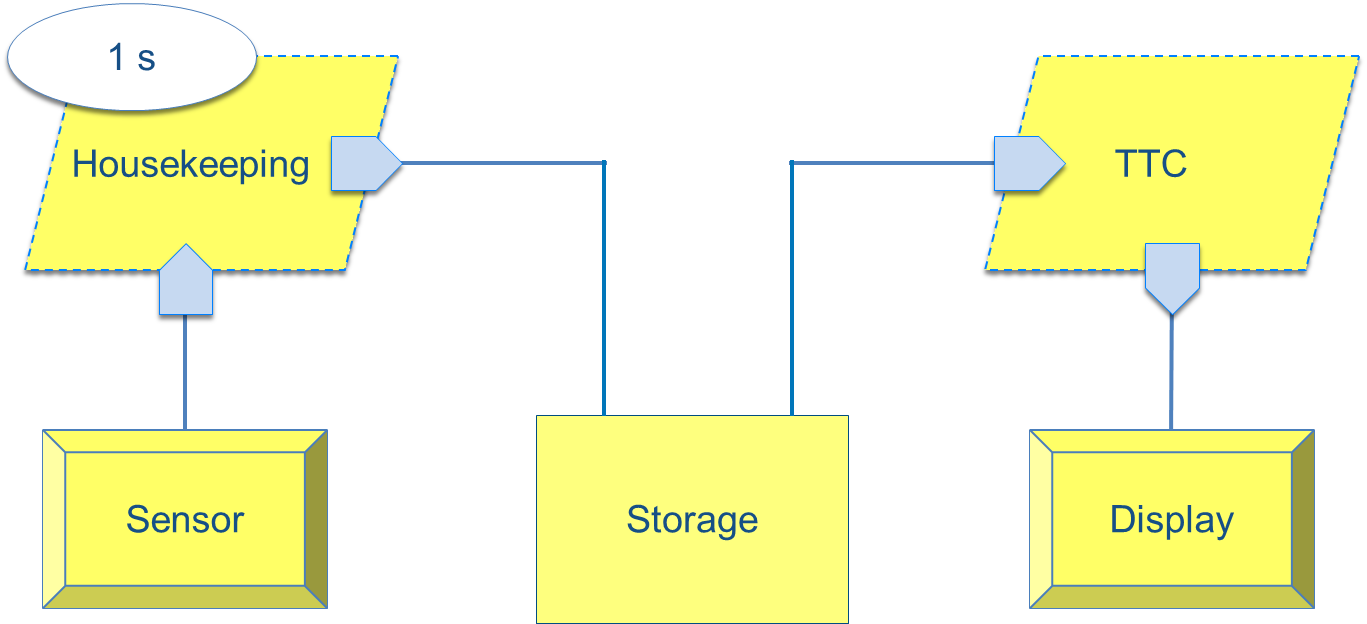
\includegraphics[width=.8\textwidth,keepaspectratio]{tasking.png}}
            \caption{Software architecture of tasking housekeeping system.}
            \label{fig:tasking}
\end{figure}

The differences with the previous architecture are:
\begin{itemize}
\item There is a new component, {\tt TTC}, that handles the display.
\item Both the {\tt Housekeeping} and {\tt TTC} components include concurrent tasks.
\item The {\tt Housekeeping} and {\tt TTC} tasks communicate through a new component, {\tt Storage}. This component is a data object storing one temperature value, which is written by {\tt Housekeeping} and read by {\tt TTC}.
\end{itemize}

\subsection{Download the code and study the implementation}

The implementation code, as initially provided to the students, can be downloaded from \url{https://github.com/STR-UPM/OBDH\_LABS}. Click on {\tt Clone} or {\tt download}, download a zip archive, unzip and move to your work directory. The code for this assignment is in the LAB4 folder.

As in the previous assignment, the {\tt Housekeeping} package is the root element of the housekeeping subsystem. Its specification and body is similar to the previous version, except that it now contains a concurrent task, {\tt Housekeeping\_Task}, and the values read from the sensor are sent to {\tt Storage} instead of {\tt Display}. This package has been moved to the {\tt TTC} subsystem, but otherwise remains similar.

The {\tt TTC} package is the root of the telecommunications system, which in this version is greatly simplified with respect to a real application. It contains a concurrent task, {\tt HK\_Task}, which takes measured sensor values from {\tt Storage} and puts them on the display.

The {\tt Storage} package implements the communication between the {\tt Housekeeping} and {\tt TTC} subsystems.  Since this object is shared by two concurrent tasks, it is implemented as a protected object, so that its operations are executed in mutual exclusion. There is also conditional synchronization: the {\tt TTC} task must wait until there is a fresh value in the store. However, {\tt Housekeeping} should not wait if the previous value put into {\tt Storage} has not been consumed, in order not to delay the housekeeping function. In this case, the stored value is overwritten. Notice that this differs from the classical specification of a bounded buffer.

The {\tt OBSW} main procedure initialises the board LEDs and the {\tt Housekeeping} and {\tt TTC} subsystems toggle blue and orange LEDs.  The activity of both subsystems is carried out by their respective tasks, which start executing concurrently with the main task. The initialization procedures return to the main procedure, which enters an endless loop doing nothing and running in parallel with the other tasks. In order not to disturb the execution of the subsystems tasks, the main loop runs at the lower possible priority, which is specified in the {\tt obsw.ads file.}

\section{Compile and run with the debugger.}

Open GPS and do the following:
\begin{enumerate}
\item Select {\tt Open project} on the welcome window. Navigate to the LAB4 directory and open the {\tt tasking\_housekeeping.gpr} project file.

\item Build the executable and load it into the board by clicking on the \hbox{
\includegraphics[width=1.5em]{debug.png}} symbol in the tool bar (or select {\tt Build} > {\tt Bareboard} > {\tt Debug} on board on the top menu).

The program will be compiled, and the executable will be loaded into the board memory by the debugger. After that, the debugger is started, and the debugger console (lowest window in GPS) shows the following lines:
\begin{verbatim}
...
(gdb) monitor reset halt
(gdb)
\end{verbatim}

\item Type {\tt continue} or just {\tt c} on the debugger console (or select {\tt Debug} > {\tt Continue} on the top menu).
\begin{verbatim}
(gdb) c
Continuing.
[program running]
\end{verbatim}

\item The program will start running (check the LED blinking), and the raw temperature readings are shown on the {\tt Messages} tab of the debugger console as in the previous project.
\end{enumerate}

\section{Make changes to the program}

You may include the same changes that were proposed in the previous assignment:

\begin{enumerate}
\item Include the conversion to Celsius in the {\tt Display.Put} procedure.
\end{enumerate}

%!TEX root = manual.tex
%===============================================================================
\chapter{Distributed housekeeping program}\label{ch:Assignment5}

The two previous versions of the housekeeping program display the measured values on a debugger console. This means that the program must be run from the debugger, with the ST-LINK cable in place.

A more realistic solution uses a serial interface to send these values to a simulated ground station running on the host computer, as shown in figure~\ref{fig:architecture}). The aim is to simulate the radio link between the satellite and the ground station.

\section{Serial line connections.}\label{sc:serial}

This scheme makes use of the USB/UART interface cable provided to the students. The USB/ UART cable has a TTL connector that must be connected to the STM32f4 board pins that convey the serial line (UART) signals (figure~\ref{fig:cable}).

\begin{figure}[h]
            \centering{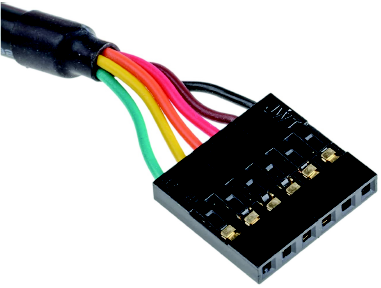
\includegraphics[width=0.3\textwidth,keepaspectratio]{connector.png}}
            \caption{UART cable connector.}
            \label{fig:cable}
\end{figure}

The connections to be made are summarized in the following table (see figure~\ref{fig:board} for the location of the pins on the board):

\begin{table}[htb]
\begin{center}
\begin{tabular}{ll} \hline
Connector pin & Board pin \\ \hline
1 (black) & GND \\
4 (orange) & PB7 \\
5 (yellow) & PB6 \\ \hline
\end{tabular}
\caption{Serial line connections on board.}
\label{tb:connections}
\end{center}
\end{table}

The other end of the interface cable has a USB-A connector that must be plugged to a USB port on the host computer. The values sent to the host computer are displayed using a terminal application that can handle a USB serial port. The host terminal application should be set to taking the USB serial port as input with a transmission rate of 115200 bps and 8N1.

\section{Host terminal application.}\label{sc:term}
\subsection{Windows}

The recommended application to display messages received on the USB serial port is PuTTY. You can download an installation package from \url{https://www.putty.org}.

In order to configure the application, you need first to identify the COM port corresponding to the USB serial line. Open the Device Manager and look at the USB Serial Port entry. The COM port is displayed next to it (e.g. COM 4 in figure~\ref{fig:com}).

\begin{figure}[h]
            \centering{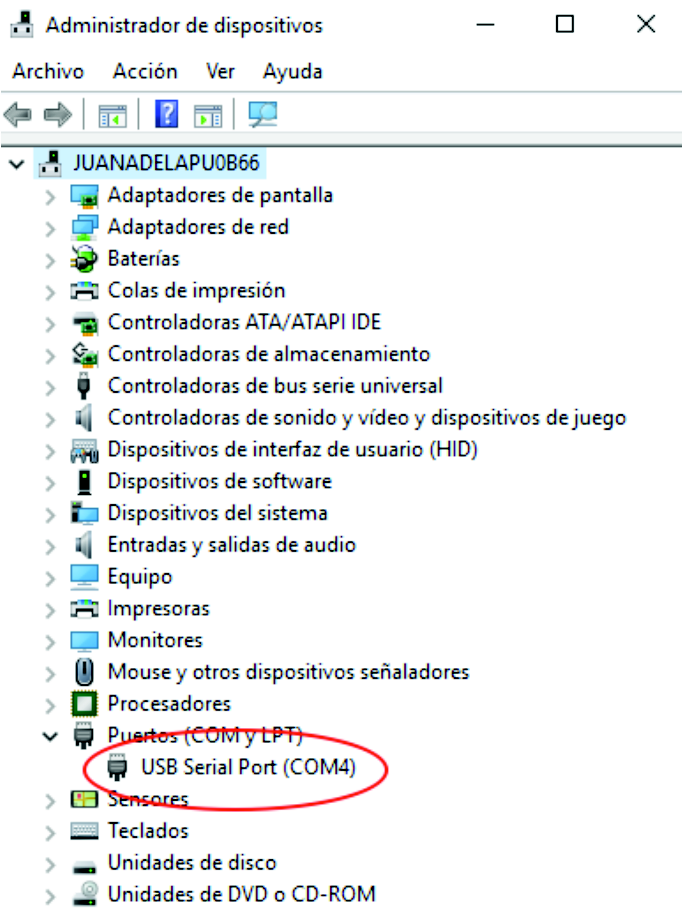
\includegraphics[width=0.6\textwidth,keepaspectratio]{com.png}}
            \caption{Identification of usb serial port.}
            \label{fig:com}
\end{figure}

Now, to set up PuTTY, open the application and set the configuration parameters as shown in figure~\ref{fig:cable}.

\begin{figure}[h]
            \centering{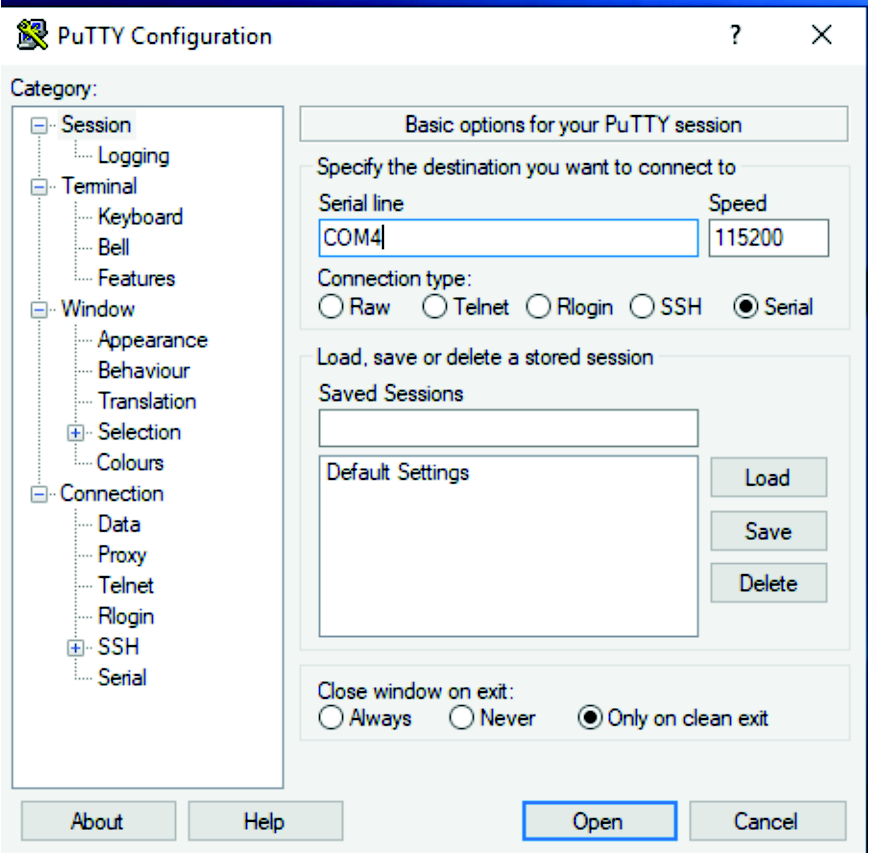
\includegraphics[width=0.6\textwidth,keepaspectratio]{putty.png}}
            \caption{PuTTY configuration.}
            \label{fig:putty}
\end{figure}

\subsection{MacOS}
The recommended application is screen, which is already installed in MacOS.
First you have to identify the USB serial port. Open a terminal window and type
\begin{verbatim}
\$ ls /dev | grep -i usb
\end{verbatim}
You will get a list of devices like the following:
\begin{verbatim}
cu.usbserial-FTA5I24G
tty.usbserial-FTA5I24G
\end{verbatim}

As you can see, there are two devices for each serial line. You can use any of them, but for reasons not to be discussed here it is better, in general, to use the one starting with cu.

To use the screen application enter the following command:
\begin{verbatim}
\$ screen /dev/cu.usbserial-XXXX 115200
\end{verbatim}

where {\tt /dev/cu.usbserial-XXXX} is the name of your device.

To exit the application, type CTRL-A and then CTRL-K.

\subsection{GNU Linux}

The recommended application is screen\footnote{{\tt gtkterm} or {\tt kermit} are good alternatives}, which can be installed in Ubuntu Linux with:
\begin{verbatim}
\$ sudo apt install screen
\end{verbatim}

In order to identify the USB serial port, type the following command on a terminal:

\begin{verbatim}
\$ ls /dev | grep -i usb
\end{verbatim}

You will get a result like the following:
\begin{verbatim}
ttyUSB0
\end{verbatim}

To use the screen application enter the following command:

\begin{verbatim}
\$ screen /dev/ttyUSB0 115200
\end{verbatim}

To exit the application, type CTRL-A and then SHIFT-K.

\section{Software architecture}

The software architecture is similar to the previous project, except that the display is replaced by a serial line handler adapted from the examples in the Ada Drivers Library.


\begin{figure}[h]
            \centering{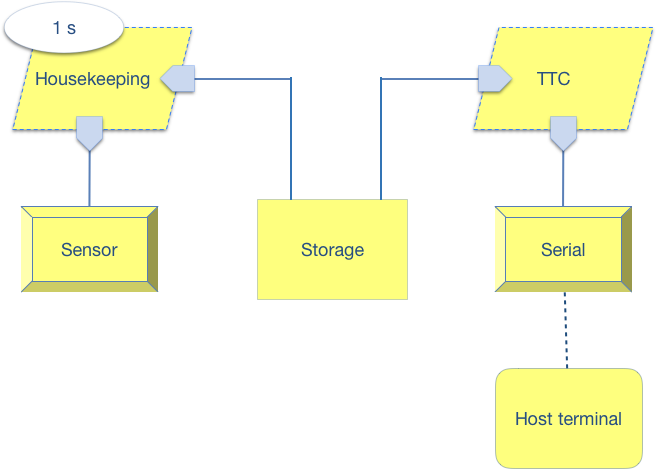
\includegraphics[width=0.6\textwidth,keepaspectratio]{distributed.png}}
            \caption{Software architecture of distributed housekeeping system.}
            \label{fig:distributed}
\end{figure}

\subsection{Download the code and study the implementation}

The implementation code, as initially provided to the students, can be downloaded from \url{https://github.com/STR-UPM/OBDH_LABS}. Click on {\tt Clone} or {\tt download}, download a zip archive, unzip and move to your work directory. The code for this assignment is in the LAB5 folder.

The {\tt Serial} component is implemented by the {\tt Serial.IO} package and other packages in the {\tt serial\_ports} folder. These packages have been adapted from the examples in the Ada Drivers Library. The blocking kind of serial port has been chosen for this project. This means that the task calling the {\tt Put} operation ({\tt TM\_Task}) waits on a busy loop until the operation is complete.

The rest of the implementation is the same as in the previous project.

\section{Compile and run.}

Open GPS and do the following:
\begin{enumerate}
\item Select {\tt Open} project on the welcome window. Navigate to the LAB5 directory and open the {\tt distributed\_housekeeping.gpr} project file.
\item Build the executable and load it into the board by clicking on the \hbox{
\includegraphics[width=1.5em]{buildandload.png}} symbol in the tool bar (or select {\tt Build} > {\tt Bareboard} > {\tt Flash to board} on the top menu).

The program will be compiled, and the executable will be loaded into the board flash memory. After that, the program starts to run on the board (check the blinking LEDs).
\item Connect the serial cable to a USB port on the host computer, if not already done.
\item Identify the serial port name on the host computer and launch the remote terminal application as explained in section~\ref{sc:term}. The sensor measured values will start being displayed on the host application.
\end{enumerate}


\section{Make changes to the program}

You may include the same changes that were proposed in the previous assignment:

\begin{enumerate}
\item Include the conversion to Celsius in the {\tt Display.Put} procedure.
\end{enumerate}

%!TEX root = manual.tex
%===============================================================================
\chapter{Real-time program}\label{ch:Assignment6}

The next version of the housekeeping program includes real-time requirements and the use of a real-time clock to add a timestamp to the housekeeping data sent to the ground station, simulated by the serial connection to the host PC like in the previous assignment. The hardware connections and the use of a host terminal application remain the same.

\section{Software architecture}

The software architecture now includes a period of 10 s for the {\tt TTC} task. This task reads the last value from the storage every 10 s (figure~\ref{fig:real-time}).

\begin{figure}[h]
            \centering{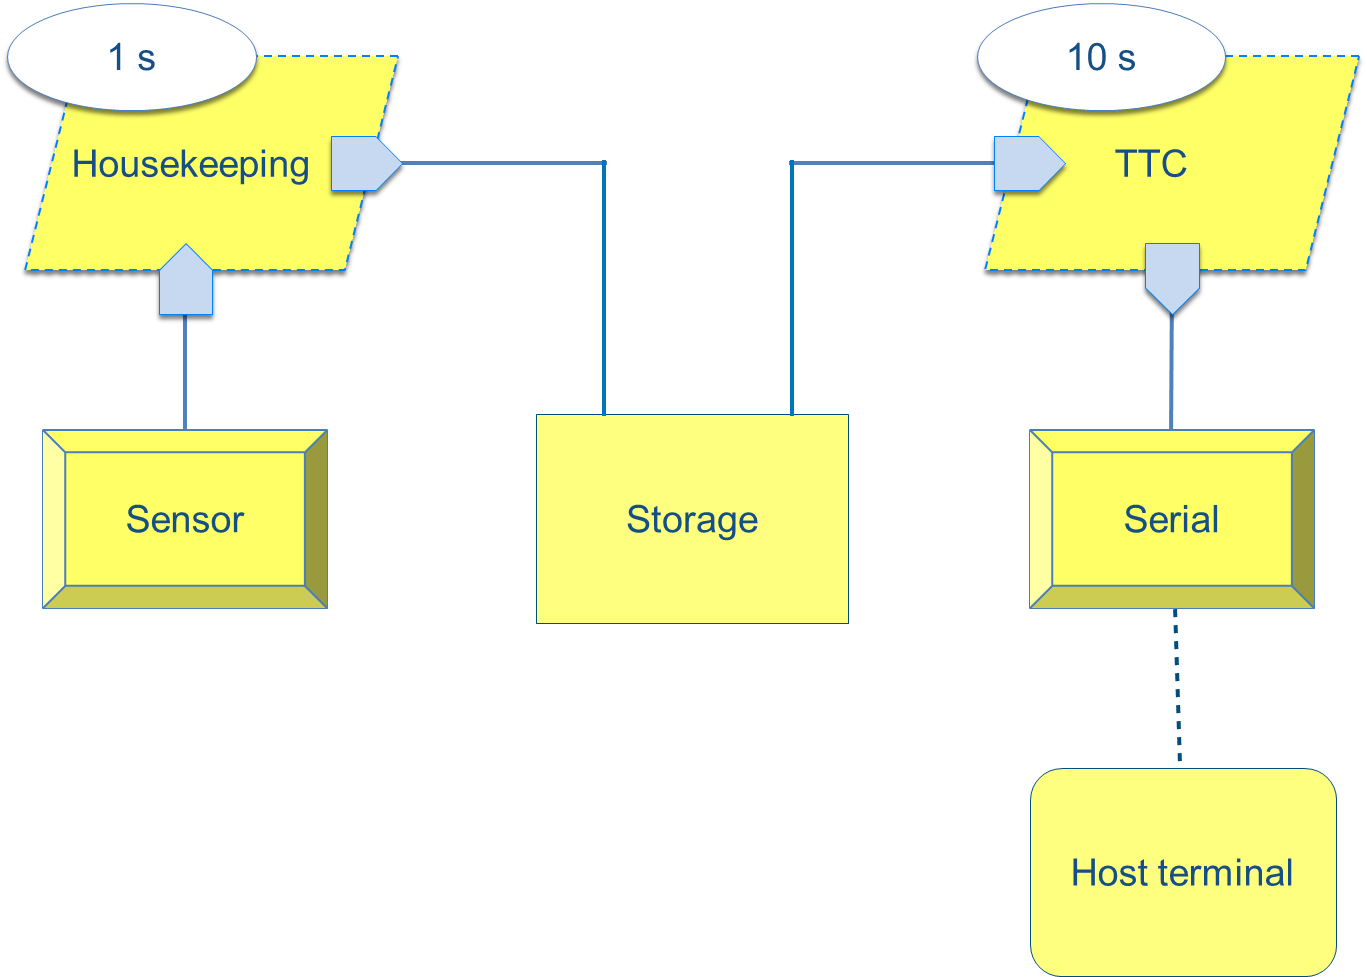
\includegraphics[width=0.8\textwidth,keepaspectratio]{real-time.png}}
            \caption{Software architecture of real-time housekeeping system.}
            \label{fig:real-time}
\end{figure}

\section{Real-time requirements}

The following real-time requirements are specified for the system:
\begin{itemize}
\item The {\tt Housekeeping} task executes with a period of 1 s and has a deadline equal to its period, (1 s).
\item The {\tt TTC} task executes with a period of 10 s and has a deadline of 2 s.
\end{itemize}

Priorities are assigned in deadline-monotonic order, as shown in table~\ref{tb:requirements}. The Buffer protected object, which is part of the {\tt Storage} implementation, is accessed by both application tasks and thus has a ceiling priority equal to the priority of the {\tt Housekeeping} task.

\begin{table}[htb]
\begin{center}
\begin{tabular}{|l|r|r|r|} \hline
Task & Period & Deadline & Priority\\ \hline
Housekeeping & 1.0 & 1.0 & 20 \\
TTC & 10.0 & 2.0 & 10 \\
Storage buffer & - & - & 20 \\ \hline
\end{tabular}
\caption{Real-time requirements.}
\label{tb:requirements}
\end{center}
\end{table}

\section{Download the code and study the implementation.}

The implementation code, as initially provided to the students, can be downloaded from \url{https://github.com/STR-UPM/OBDH\_LABS}. Click on {\tt Clone} or {\tt download}, download a zip archive, unzip and move to your work directory. The code for this assignment is in the LAB6 folder.

The implementation code differs from the previous project in several aspects.
\begin{itemize}
\item Period and priority values have been explicitly added to the specification of the {\tt Housekeeping} and {\tt TTC} packages. A start delay has been added to the respective tasks, in order to let all the packages initialize before the regular operation of the system starts.
\item The ceiling priority of the {\tt Storage} buffer has been set to the same value as the {\tt Housekeeping} task.
\item A new {\tt State} data type has been defined, which is a record including a timestamp and an analog data value. Messages sent to ground are now of this data type.

Timestamps are refined as 64-bit integers, denoting the number of second elapsed since the beginning of the mission. To the purpose of this laboratory this value is taken from the real-time clock provided by the {\tt Ada.Real\_Time} library package.
\item In order to improve the visual aspect of the messages as viewed on the host terminal application, a new package, {\tt Data\_Images}, has been added that provides fixed-width string images of mission time and analog data values.
i\end{itemize}

The rest of the implementation is the same as in the previous project.

\section{Compile and run.}

Open GPS and do the following:
\begin{enumerate}
\item Select {\tt Open} project on the welcome window. Navigate to the LAB6 directory and open the {\tt realtime\_housekeeping.gpr} project file.
\item Build the executable and load it into the board by clicking on the \hbox{
\includegraphics[width=1.5em]{buildandload.png}} symbol in the tool bar (or select {\tt Build} > {\tt Bareboard} > {\tt Flash to board} on the top menu).

The program will be compiled, and the executable will be loaded into the board flash memory. After that, the program starts to run on the board (check the blinking LEDs).
\item Connect the serial cable to a USB port on the host computer, if not already done.
\item Identify the serial port name on the host computer and launch the remote terminal application as explained in section~\ref{sc:term}.  The sensor measured values together with their respective timestamps will start being displayed on the host application (figure~\ref{fig:output}).
\end{enumerate}

\begin{figure}[h]
            \centering{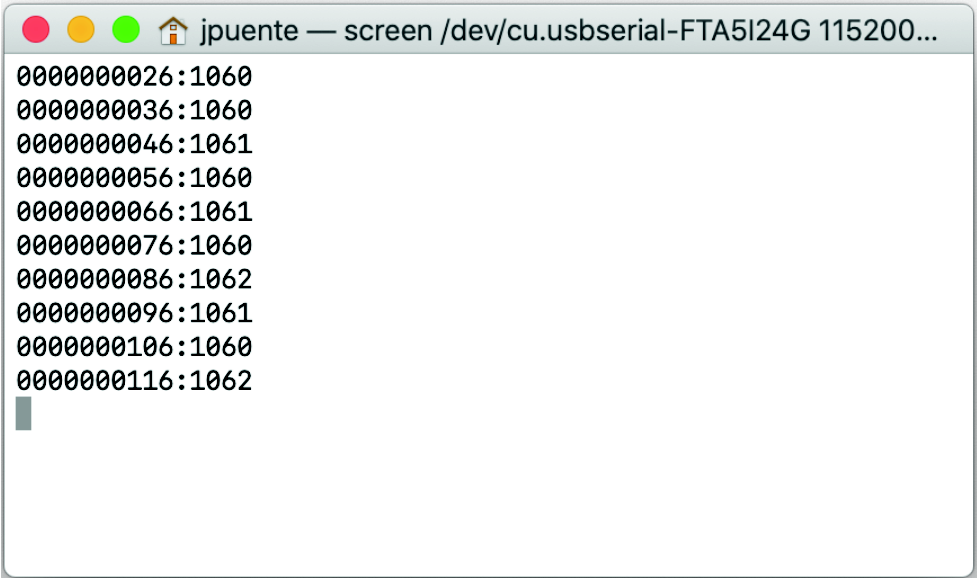
\includegraphics[width=0.6\textwidth,keepaspectratio]{output.png}}
            \caption{Sample output on host terminal.}
            \label{fig:output}
\end{figure}

\section{Perform a temporal analysis of the system.}\label{sc:ta}

In order to carry out a response-time analysis of the temporal behaviour of the system, you will need to measure the execution time of the task bodies and the protected procedure bodies. A simple loop technique using the standard real-time clock will be enough for this assignment.

An execution time measurement tool is available in the LAB6 directory. In order to use it, perform the following steps:
\begin{enumerate}
\item Open GPS and select {\tt Open} project on the welcome window. Navigate to the LAB6 directory and open the {\tt wcet\_meter.gpr} project file.
\item Build the executable and load into the board in the same way as for the realtime\_housekeeping.gpr project.
\item Make sure that the serial cable is still connected to the board and the USB port in the host computer. If the remote terminal application is not open, open it.
\end{enumerate}

A measurement test is executed on the board, and repeated every 60 s. The output of the test is shown on the host terminal application (figure~\ref{fig:wcet}). The output shows the execution times for the bodies of the {\tt Housekeeping} (HK) and {\tt TTC} (TC) tasks, as well as the bodies of the protected operations of the {\tt Storage} object (ST). Notice that a new entry, {\tt Get\_Immediate}, has been added for the latter in order to avoid the measuring task to get blocked. The new entry is exactly the same as {\tt Get} but has a {\tt True} barrier so that it is always open.

\begin{figure}[h]
            \centering{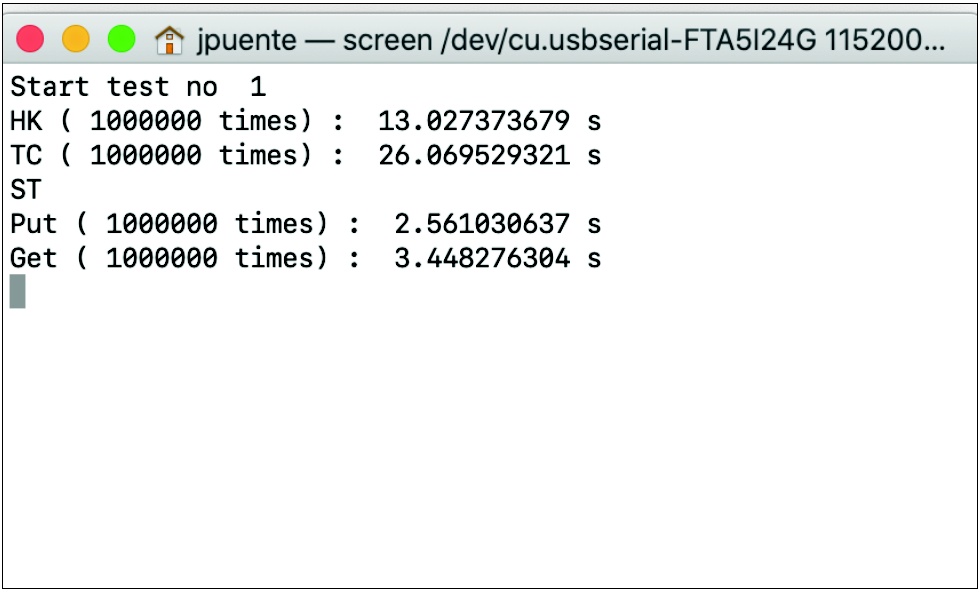
\includegraphics[width=0.6\textwidth,keepaspectratio]{wcet.png}}
            \caption{Output of wcet measurement tool.}
            \label{fig:wcet}
\end{figure}

In the example shown on figure~\ref{fig:wcet}, the HK execution time has been measured $10^{6}$ times, with a total measurement time of 13.02 s. Therefore, the value to be taken for the response time analysis is $13.02\cdot10^{-6}~s = 13.02~\mu${s}, and the same for the other tasks. Take into account that the values measured on your board will probably be slightly different from the above shown.

Once you have an estimate of worst case execution times, apply the RTA equations for computing the worst-case response time and check if all the deadlines are met. The setup for the calculations is shown on table~\ref{tb:wcet}.

\begin{table}[htb]
\begin{center}
\begin{tabular}{|l|r|r|r|r|r|r|r|r|} \hline
Task & T & C & B & D & R & P & CPut & CGet\\ \hline
Housekeeping & 1.0 & $13\cdot10^{-6}$ & $4\cdot10^{-6}$ & 1.0 & $17\cdot10^{-6}$& 20 & $3\cdot10^{-6}$ & - \\
TTC & 10.0 & $26\cdot10^{-6}$ & 0 & 2.0 & $39\cdot10^{-6}$ & 10 & - & $4\cdot10^{-6}$ \\ \hline
& & & & & & CP & 20 & 10 \\ \hline
\end{tabular}
\caption{Data arrangement for RTA of the housekeeping system.}
\label{tb:wcet}
\end{center}
\end{table}

\chapter{Real-time program with Attitude Control System}\label{ch:assignment7}

The aim of this assignment is to validate the Attitude Control System (ACS) following the Processor In the Loop (PIL) approach. The real-time version of the On-Board Software (OBSW) is used with the ACS of the UPMSat-2 satellite. The ACS uses magnetic sensors and actuators, which is commonly known as magnetic attitude control (figure~\ref{fig:acs}).

\begin{figure}[h]
            \centering{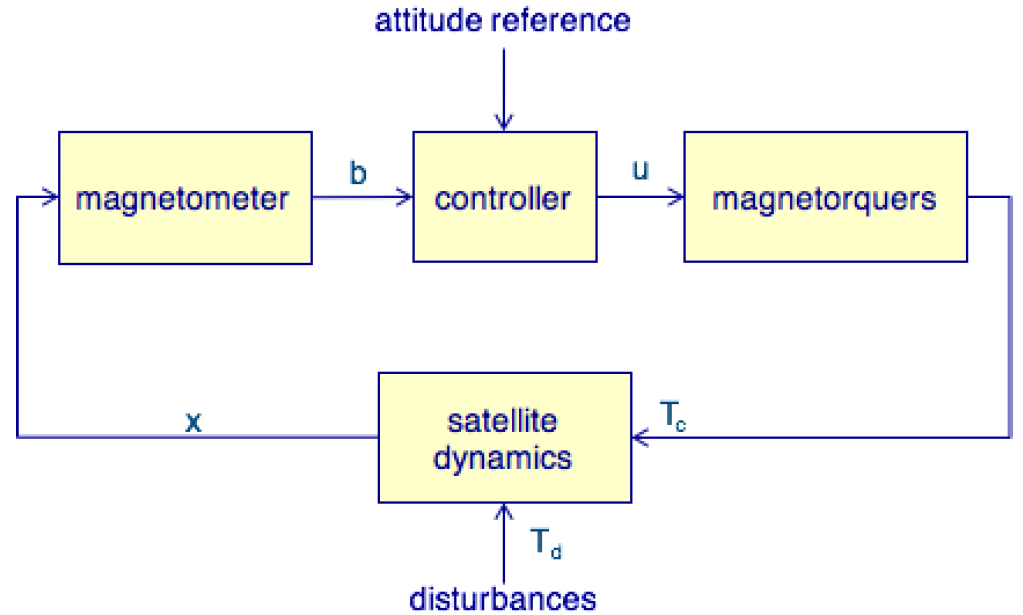
\includegraphics[width=.6\textwidth,keepaspectratio]{acs.png}}
            \caption{Magnetic attitude control system.}
            \label{fig:acs}
\end{figure}

Magnetometers are magnetic sensors that provide a measurement of the strength and direction of the magnetic field, i.e. the magnetic field vector, at a given point. Magnetorquer are magnetic coil which produce a magnetic moment that interacts with the Earth's field, thus enabling the attitude of the satellite to be changed.

\section{Model In the Loop (MIL) validation}

Software validation usually includes testing the system under real operating conditions. However, for obvious reasons, on-board space software as well as many other embedded systems cannot be tested in this way. Simulation models are commonly used in these cases.

The first validation phase uses a model of the ACS, together with models of the space environment and the spacecraft dynamics, to assess the validity of the control law and the design parameters (figure~\ref{fig:acs-hl}). This is usually carried out by a control engineer using a simulation tool. Simulink is commonly used for ACS development.

\begin{figure}[h]
            \centering{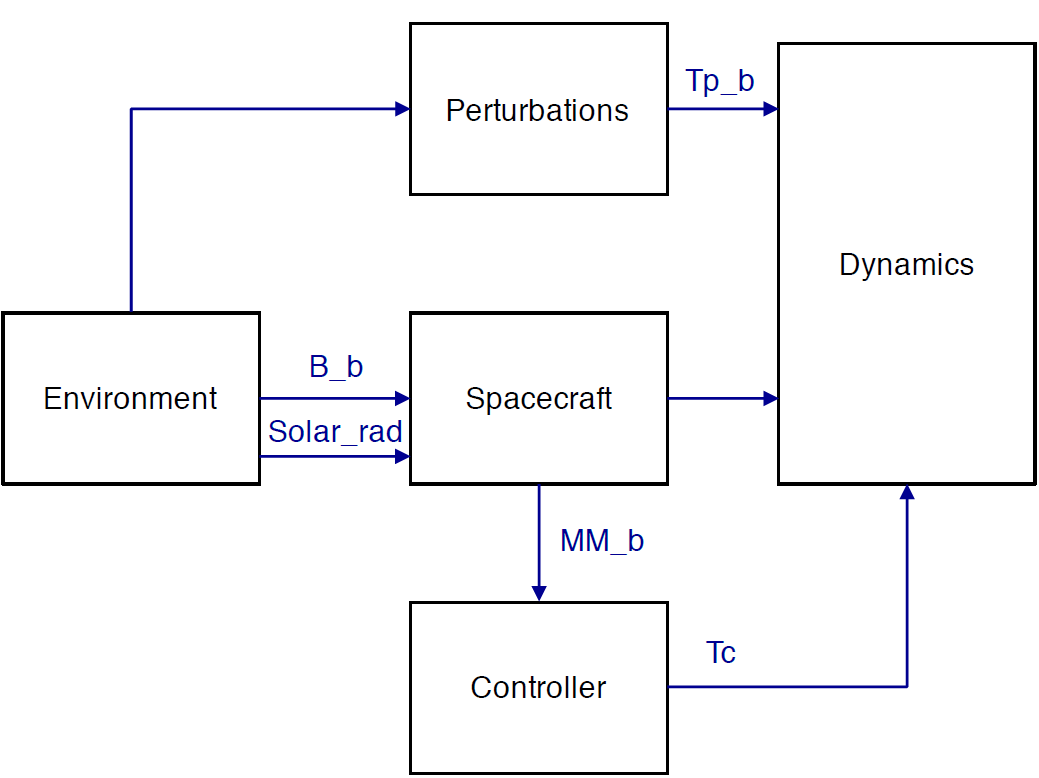
\includegraphics[width=0.6\textwidth,keepaspectratio]{acs-hl.png}}
            \caption{UPMSat-2 ACS high level model view.}
            \label{fig:acs-hl}
\end{figure}

The ACS simulink model can be simulated by running {\tt matlab} from directory LAB7/ACS and opening ACS.slx. Three new windows will be pop-up: the simulink window with the ACS model and two scope windows that show the angular velocity of the satellite in body reference and the actuation over the three magnetorquers.

The simulink window (figure~\ref{fig:acs-simulink}) shows the high level blocks, that are the satellite itself, its dynamic and the models of the Earth's field and Sun with the perturbations.

\begin{figure}[h]
            \centering{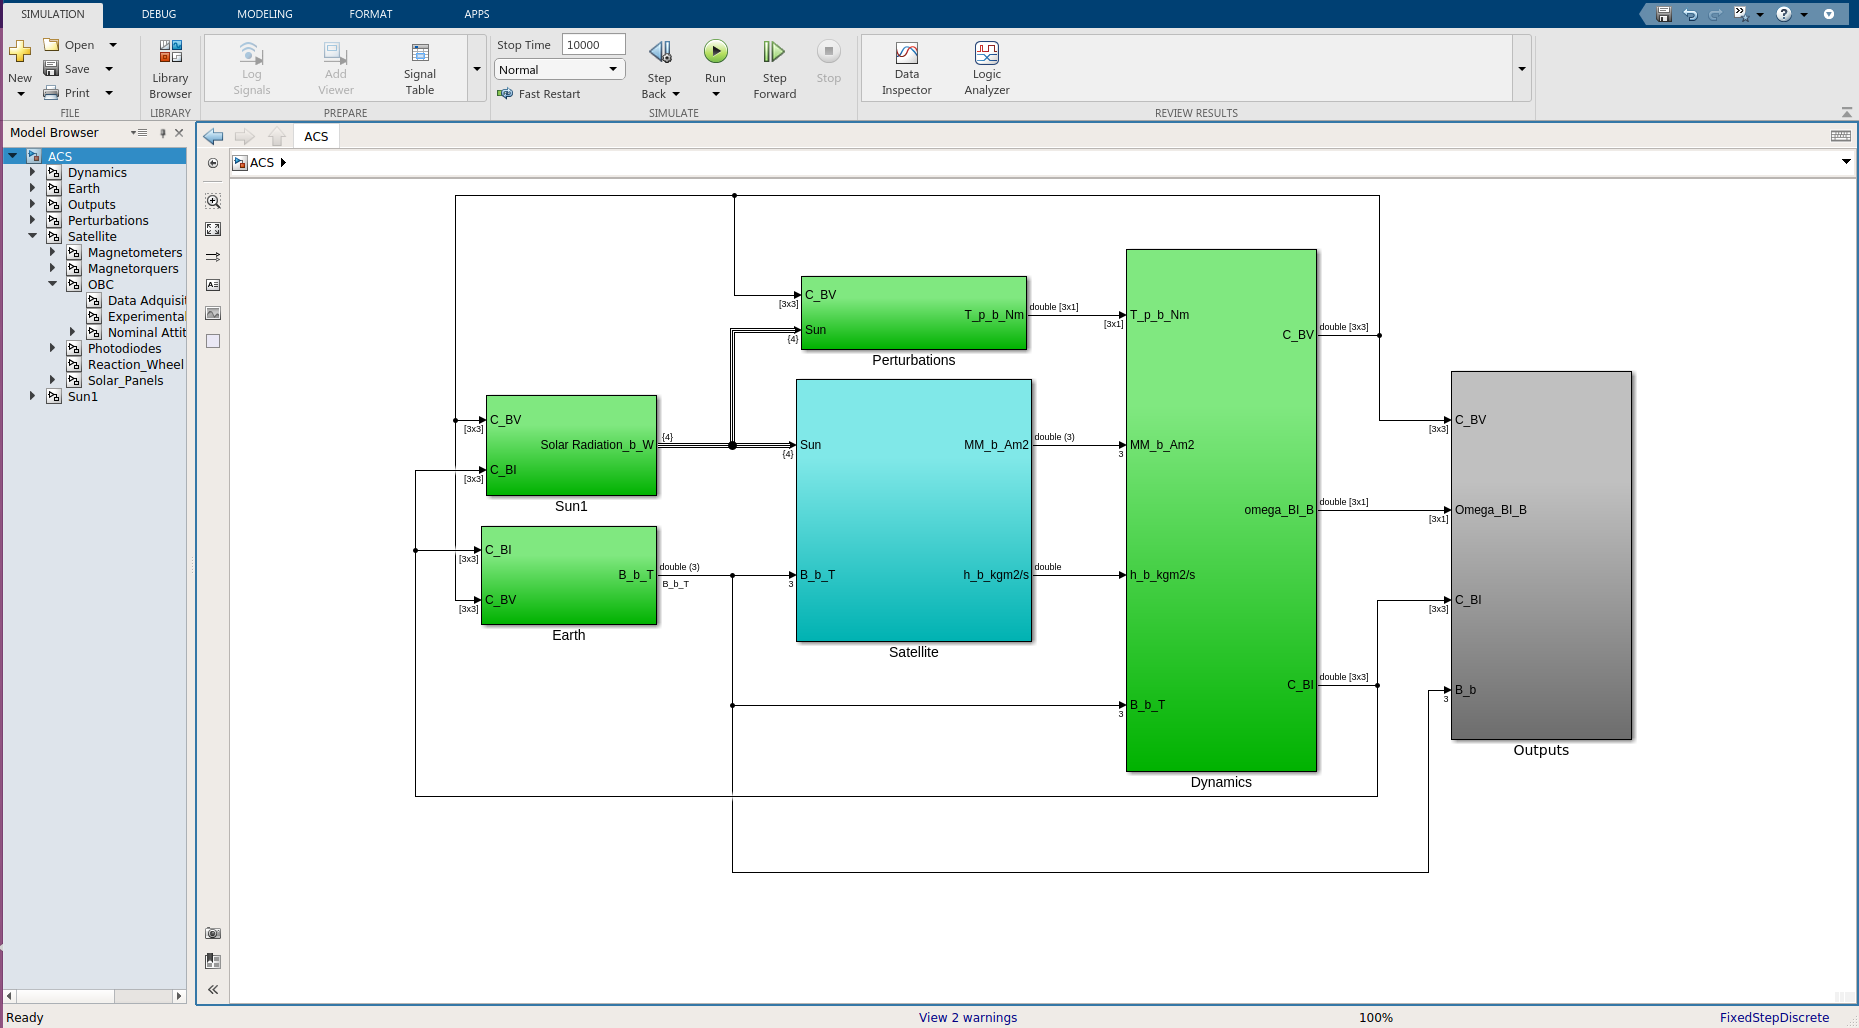
\includegraphics[width=\textwidth,keepaspectratio]{acs-simulink.png}}
            \caption{UPMSat-2 simulink model.}
            \label{fig:acs-simulink}
\end{figure}

The nominal attitude control can be show by selecting {\tt Nominal Attitude Control} in the Model Browser menu (left part of simulink window) or by clicking on {\tt Satellite} > {\tt OBC} > {\tt Nominal Attitude Control} blocks.

Nominal attitude control has three blocks (figure~\ref{fig:nac}):
\begin{description}
\item[Sensor] samples the analog inputs of the magnetometers. The inputs are converted to engineering units using calibration data.
\item[Control] implements the attitude control law that computes the control action to be output to the magnetorquers.
\item[Actuator] activates the magnetorquers according to the computed control action.
\end{description}

\begin{figure}[H]
            \centering{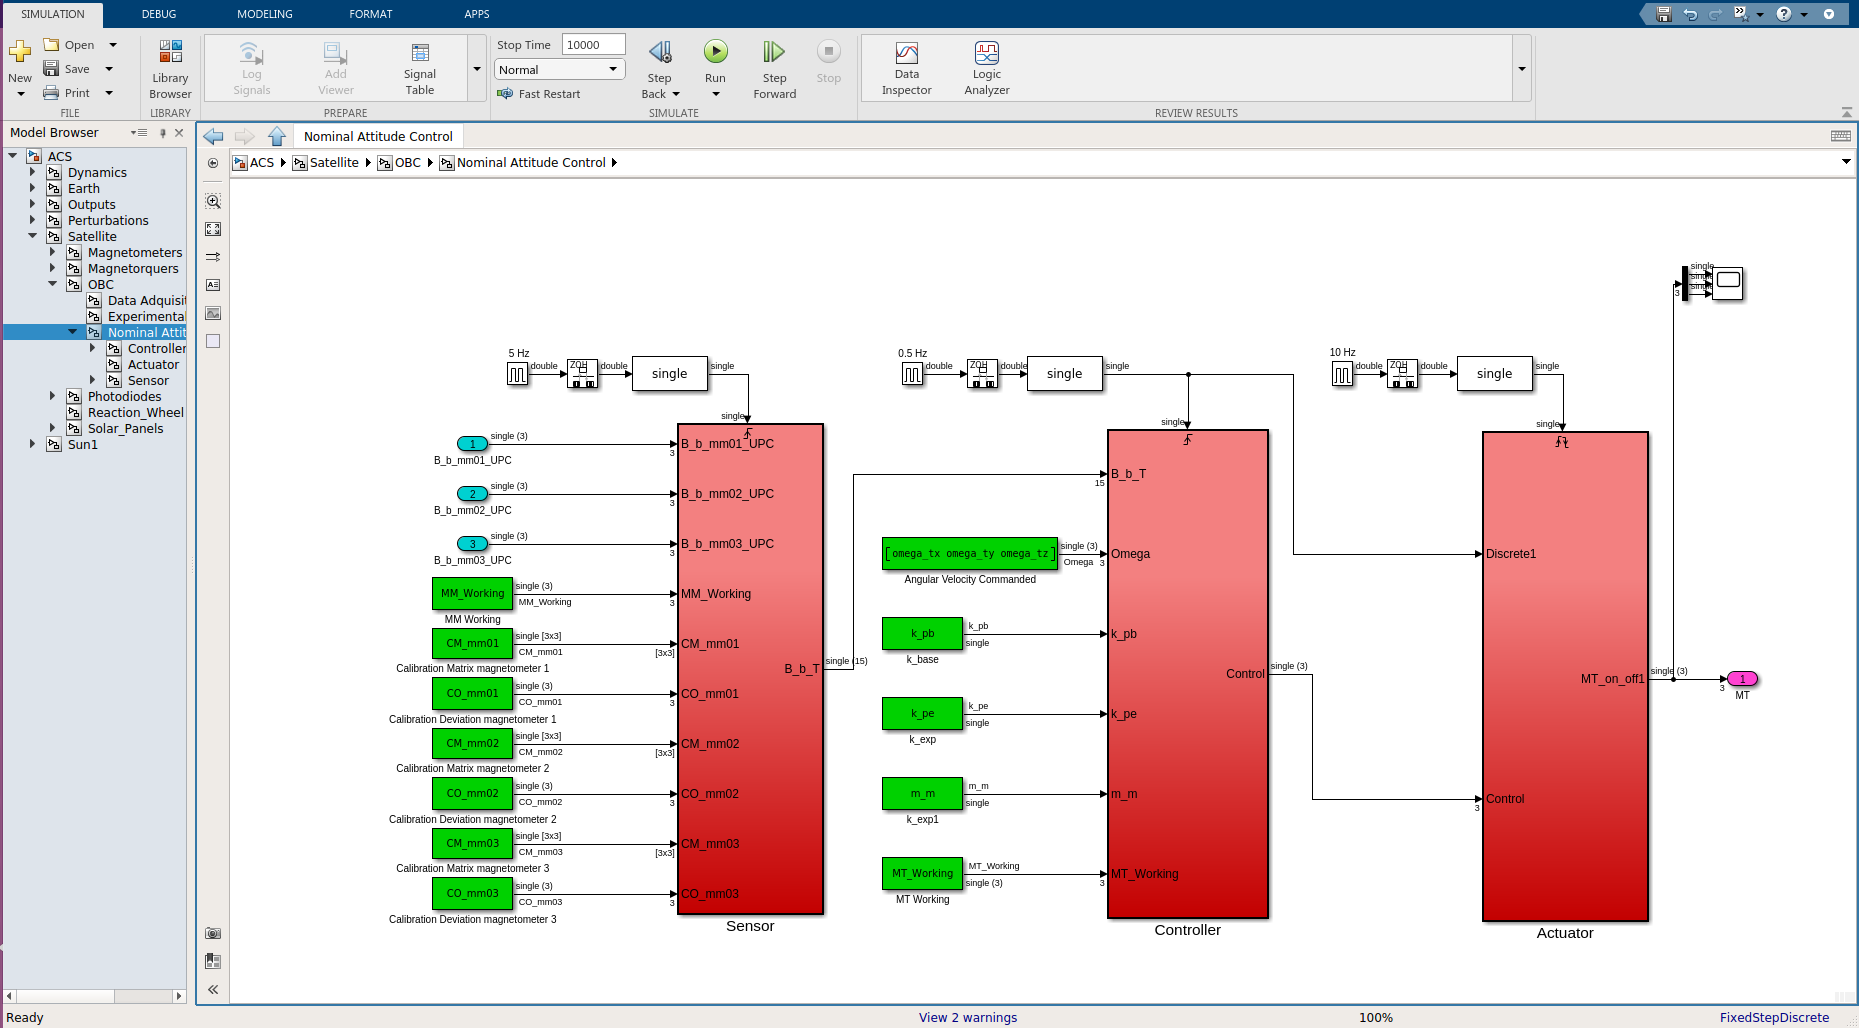
\includegraphics[width=\textwidth,keepaspectratio]{nac.png}}
            \caption{Nominal attitude control.}
            \label{fig:nac}
\end{figure}

To simulate the model an verify its behaviour, click on {\tt Run} bottom. The evolution of the angular velocity of the satellite and the actuation over the three magnetorquers will be shown in the corresponding scope windows. The commanded angular velocity is [0, 0, 0.1] rad/s and the result of the simulation (figure~\ref{fig:scope}) shows that evolution from the initial angular velocity ([0.1, -0.1, -0.1] rad/s).

\begin{figure}[h]
            \centering{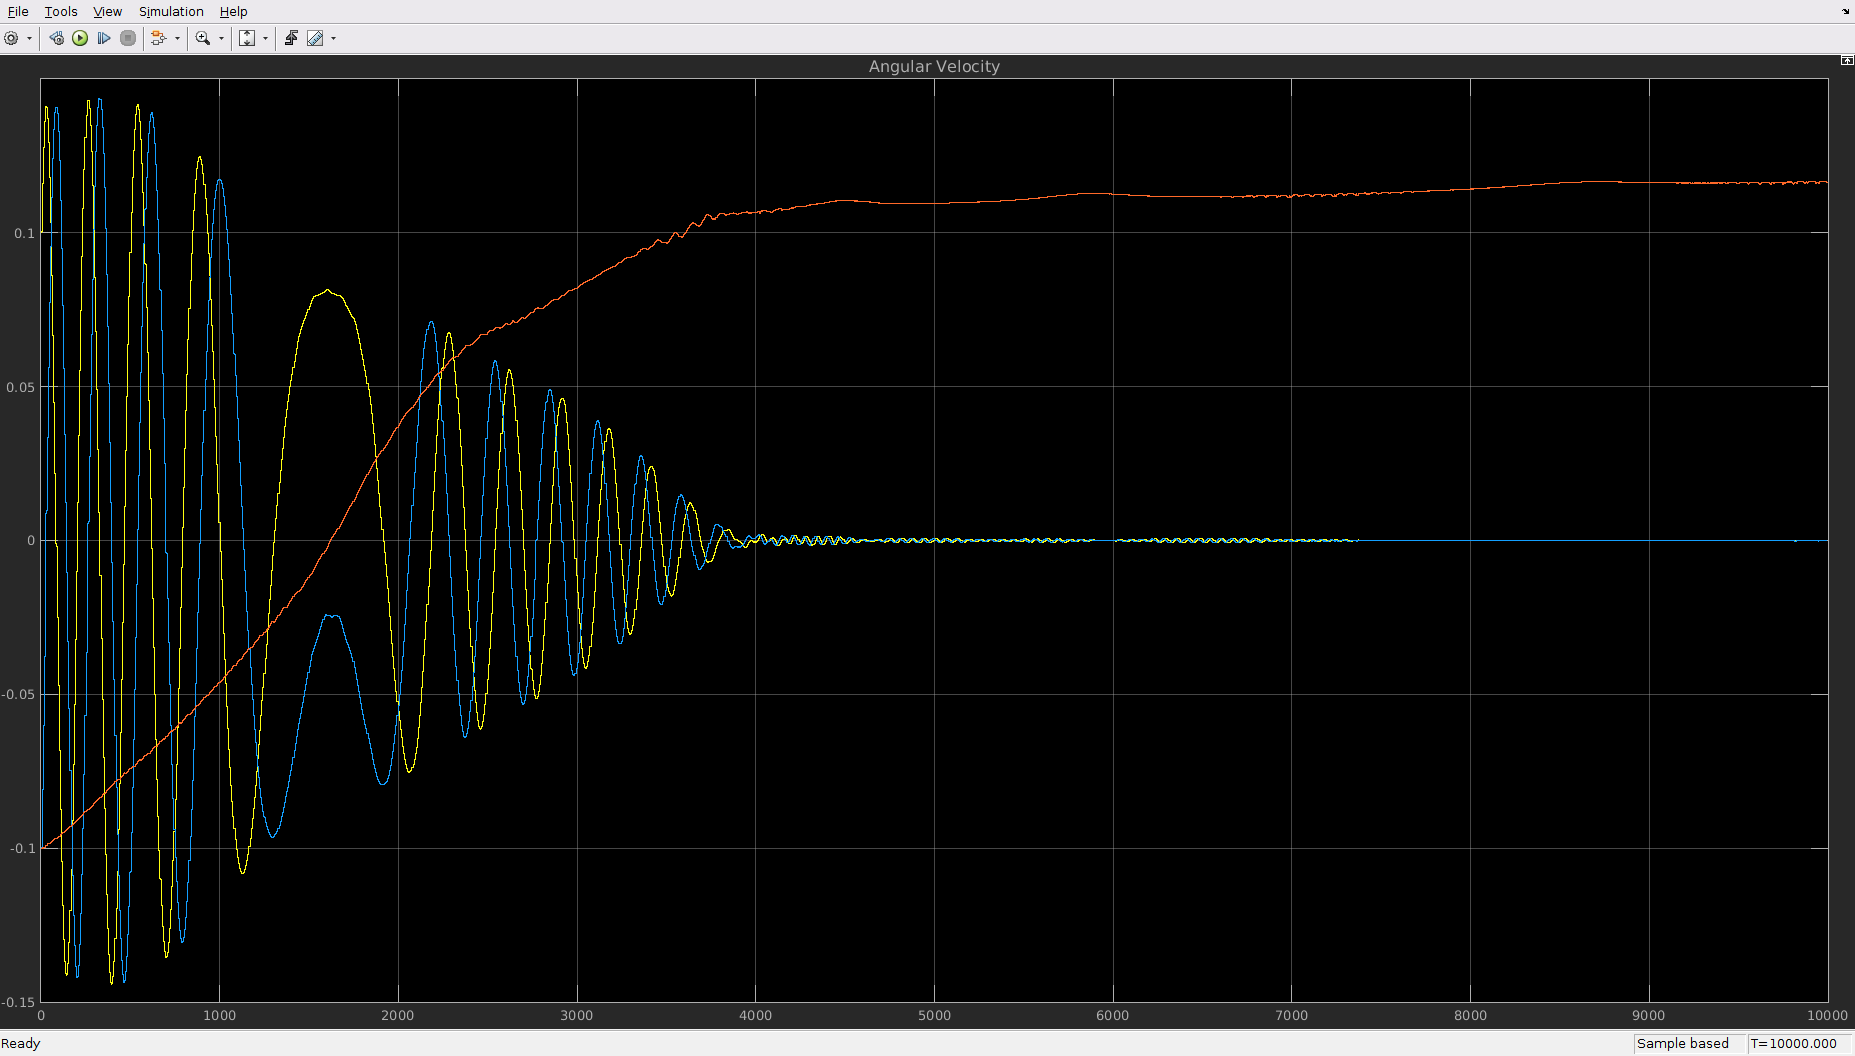
\includegraphics[width=\textwidth,keepaspectratio]{scope.png}}
            \caption{Angular velocity evolution.}

            \label{fig:scope}
\end{figure}

\section{Code generation.}

The next step is execute the ADCS on hardware. In this assignment, only the Control block will be execute on the target board.
The corresponding code can be generated by using the Embedded Coder toolbox but it is needed to isolate Control block from the ACS model. It can be done by clicking in the Control block, selecting all the block content (except the trigger block) and saving it in a new model. 

This model named control.slx can be found in LAB7/ACS\_PIL directory. Use {\tt matlab} to open it and then select {\tt APPS} in the top menu, {\tt Embedded Coder} will appear. If not, it must be installed by clicking {\tt Get Add-Ons} and searching it. The Embedded Coder window (figure~\ref{fig:control}) will appear after clicking on Embedded Coder icon.

\begin{figure}[h]
            \centering{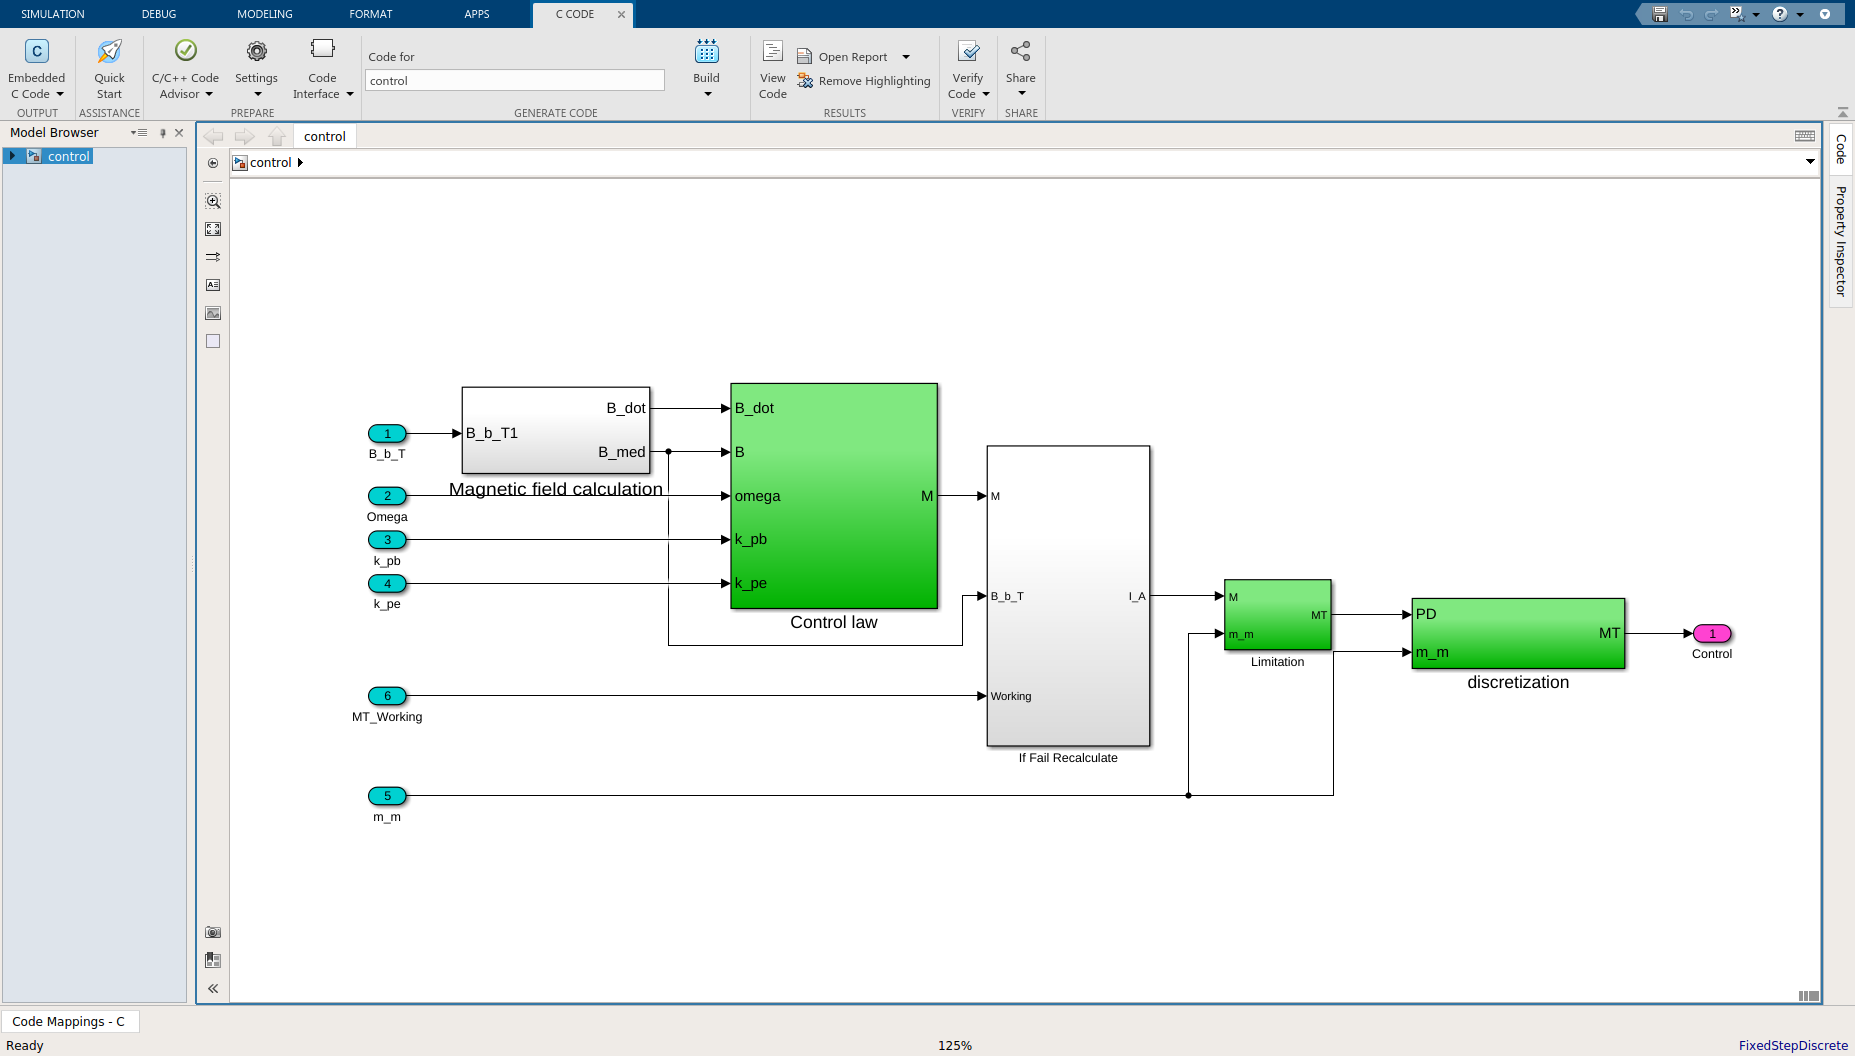
\includegraphics[width=\textwidth,keepaspectratio]{control.png}}
            \caption{Embedded Coder toolbox.}

            \label{fig:control}
\end{figure}

The code generation option as well as characteristics of the target hardware can be set by clicking on the {\tt Settings} menu. {\tt control.slx} model has already the proper options, therefore you can take a look but be carefully and do not modify then.

Now the code can be generated by clicking on the {\tt Build} menu. Once upon the code is generated, a code generation report window appear. It is possible to explore the generated code together with different code metrics. Click on {\tt control.h} and look for lines 50-79 (figure~\ref{fig:code}) where the generated code interface is located.

\begin{figure}[h]
            \centering{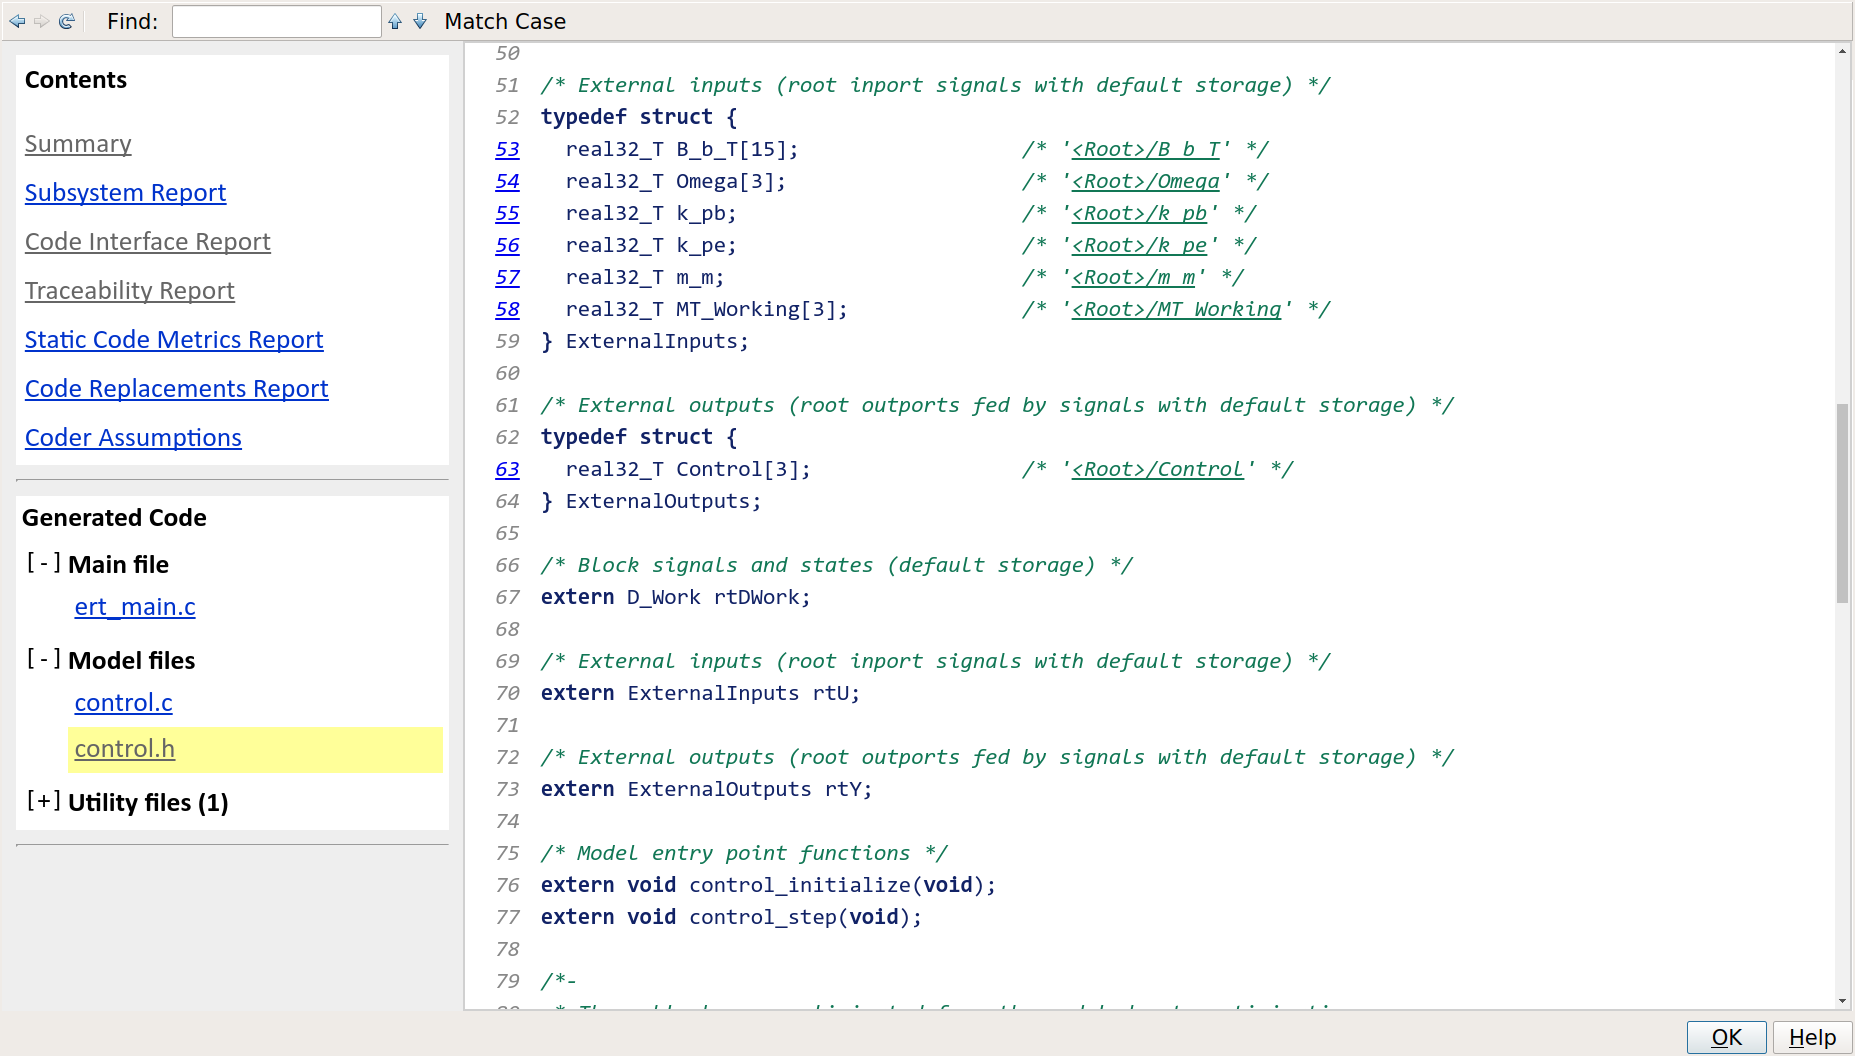
\includegraphics[width=\textwidth,keepaspectratio]{code.png}}
            \caption{Code generation report.}

            \label{fig:code}
\end{figure}

There are two record type definitions ({\tt struct}) called {\tt ExternalInputs} and {\tt ExternalOutputs} that are used to interchange data with the blocks {\tt Sensor} and {\tt Actuator} (figure~\ref{fig:nac}). Data are interchanged with two objects of these record types: {\tt rtU} and {\tt rtY}. There are also two functions: function {\tt control\_initialize} initializes the control code and function {\tt control\_step} performs the control algorithm.

The generated code will be embedded in the real-time program by taking into account this interface.

\section{Software architecture}

The implementation code, as initially provided to the students, can be downloaded from \url{https://github.com/STR-UPM/OBDH\_LABS/LAB7}.

\begin{figure}[H]
            \centering{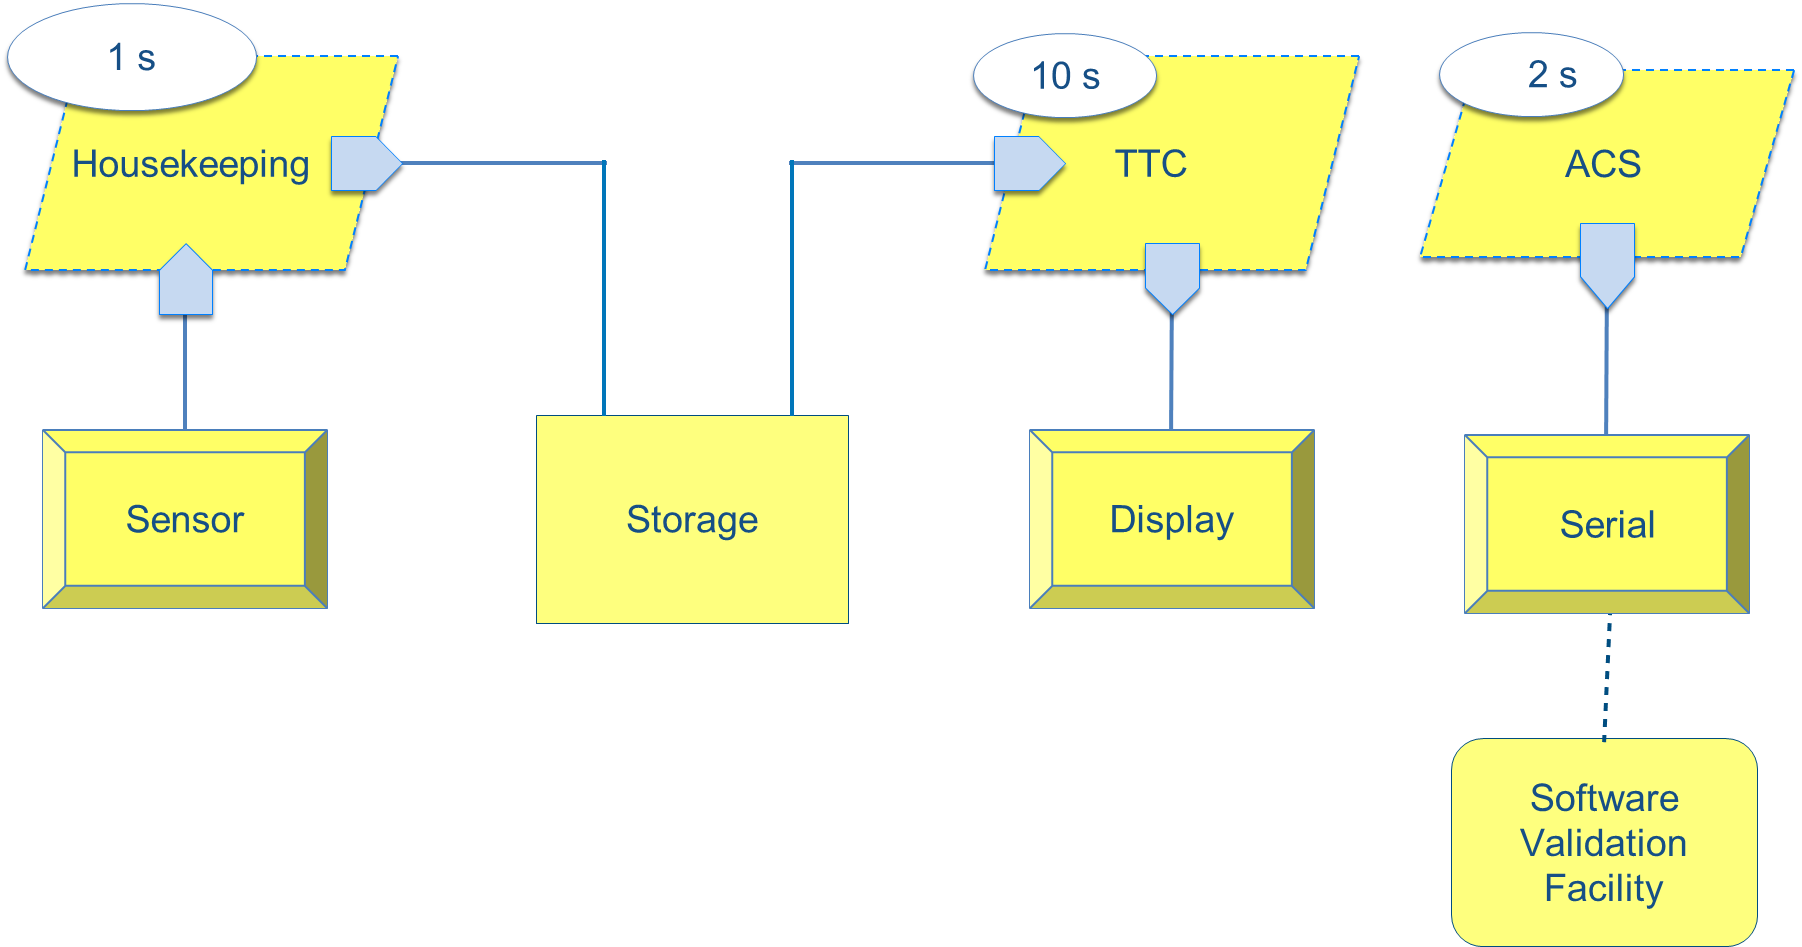
\includegraphics[width=\textwidth,keepaspectratio]{obsw-acs.png}}
            \caption{Software architecture of the real-time program with ACS.}
            \label{fig:obdh-acs}
\end{figure}

The software architecture of the the real-time program with ACS is depicted in figure~\ref{fig:obdh-acs} and the differences with the previous architecture (figure~\ref{fig:real-time}) are:

The {\tt ADCS} package is the root element of the ADCS. Its specification consists of one procedure, {\tt Initialize}, that starts the operation of the component. It has three subpackages:
\begin{description}
\item[ADCS] is the root package of the subsystem and contains a concurrent task, {\tt ADCS\_Task} that reads the magnetic field vector from {\tt Sensor}, calculates the actuation vector and sends it to {\tt Actuator} (see figure~\ref{fig:nac}). It also toggles the red LED every two second.

The body of this package uses the generated code by setting the inputs, calling the functions and retrieving the outputs following the interface of figure~\ref{fig:code}. {\tt ADCS\_Task} performs the control algorithm by calling {\tt control\_step}. This is shown in figure~\ref{fig:acs-body}.
It uses {\tt Export} and {\tt Import} pragmas to interface the generated C code.

\begin{figure}[h]
            \centering{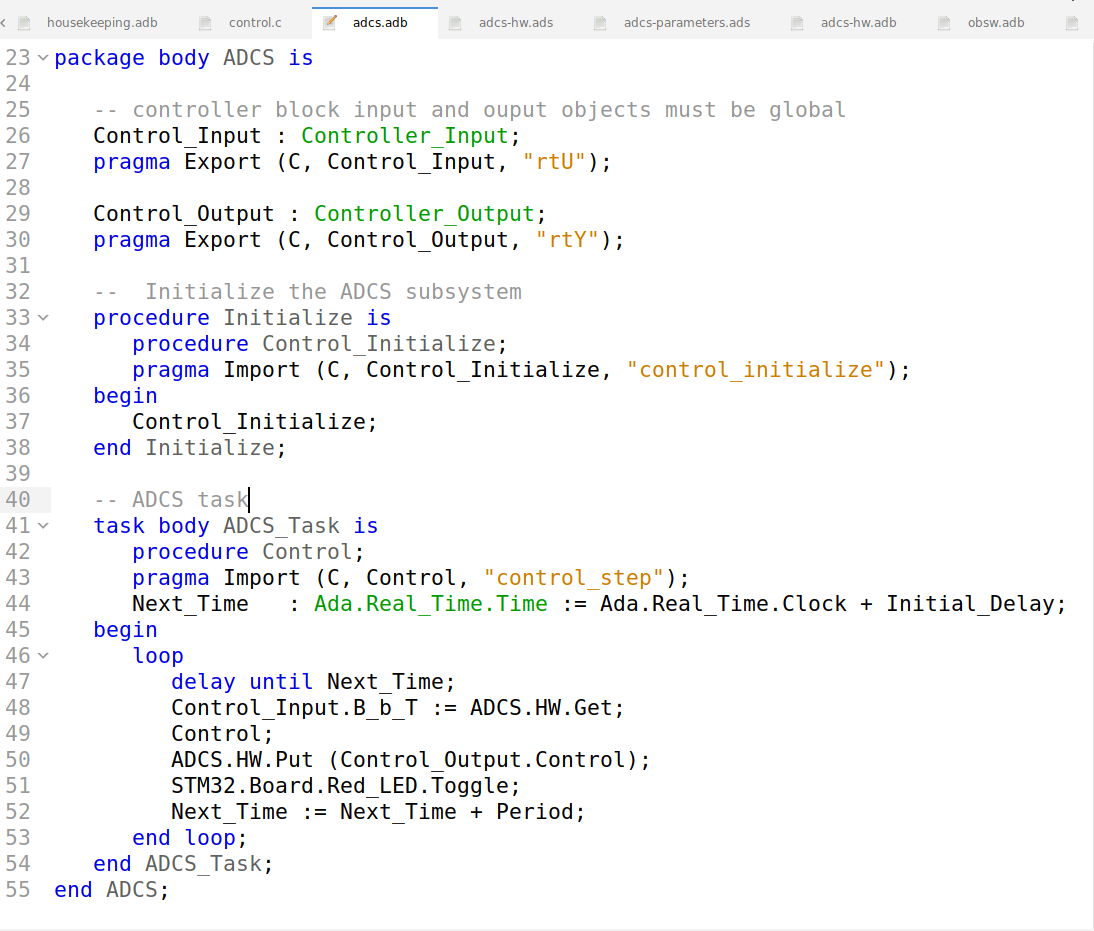
\includegraphics[width=\textwidth,keepaspectratio]{acs-body.png}}
            \caption{Implementation of ACS package.}
            \label{fig:acs-body}
\end{figure}

\item[ADCS.Parameters] contains the definitions of the data types used in the subsystem and parameters that are used to tune the control algorithm. These parameters can be changed by telecommand in the UPMSat-2 OBSW. The data type {\tt Controller\_Input} is used to read the magnetic field vector in teslas, which are IEEE single precision float numbers. The data type {\tt Controller\_Output} are used to send the actuation to magnetorquers in seconds\footnote{In UPMSat-2 ACS, Pulse Width Modulation (PWM) is used. Therefore outputs are the duration of actuations (duty cycles) on magnetorquers and resulting units are joule-seconds.}, which are IEEE single precision float numbers. These data types correspond to the generated C structs {\tt ExternalInputs} and {\tt ExternalOutputs} (see figure~\ref{fig:code}).

\item[ADCS.HW] is in charge of getting the magnetic field vector and putting the
actuations. It hides the details of the hardware. Its specification includes the {\tt Put} and {\tt Get} subprograms. This package uses the serial port to interchange magnetic field and actuation values with the Software Validation Facility.
\end{description}

The Software Validation Facility (SVF) is an auxiliary computer, linked to the OBC by a serial line, to run a simulation model of the Earth's magnetic field and satellite dynamics. In this way, engineering values can be interchanged.
Host computers are also used as SVF by executing a Simulink\texttrademark model of the Earth's magnetic field and satellite dynamics.

In this assignment, the serial line is used to interchange data between ADCS and SVF. Therefore, housekeeping telemetry are send to a text console that is simulated on the host computer using semihosting as in assignments 3 and 4.

\section{Compile and run with the debugger.}

Open GPS and do the following:
\begin{enumerate}
\item Select {\tt Open project} on the welcome window. Navigate to the LAB7 directory and open the {\tt realtime\_housekeeping.gpr} project file.
\item Build the executable and load it into the board using the debugger by clicking on the \hbox{
\includegraphics[width=1.5em]{debug.png}} symbol in the tool bar (or select {\tt Build} > {\tt Bareboard} > {\tt Debug} on board on the top menu).

The program will be compiled, and the executable will be loaded into the board memory by the debugger. The debugger console (lowest window in GPS) shows the following lines:
\begin{verbatim}
...
(gdb) monitor reset halt
(gdb)
\end{verbatim}

\item Type {\tt continue} or just {\tt c} on the debugger console (or select {\tt Debug} > {\tt Continue} on the top menu).
\begin{verbatim}
(gdb) c
Continuing.
[program running]
\end{verbatim}

After that, the program starts to run on the board and temperature reads are displayed on messages tab of the debugger window. However, the red LED does not blink because {\tt ACS} is waiting sensor inputs from SVF.
\end{enumerate}

\section{Processor In the Loop (PIL) validation.}

The SVF shall provide sensor inputs and retrieve magnetotorquer outputs. To do that, the remain part of the original simulink model will be used, i.e. all the blocks except the Sensor block.

This model named {\tt ACS\_PIL.slx} can be found in LAB7/ACS\_PIL directory. Open it and again three new windows will be pop-up: the simulink window with the ACS\_PIL model and two scope windows that show the angular velocity of the satellite in body reference and the actuation over the three magnetorquers.

The Control block of this model has been substituted by serial link connections as shown in figure~\ref{fig:nac-pil}. Identify the serial port name on the host computer and edit the serial configuration block by selecting the serial line of your PC.

\begin{figure}[h]
            \centering{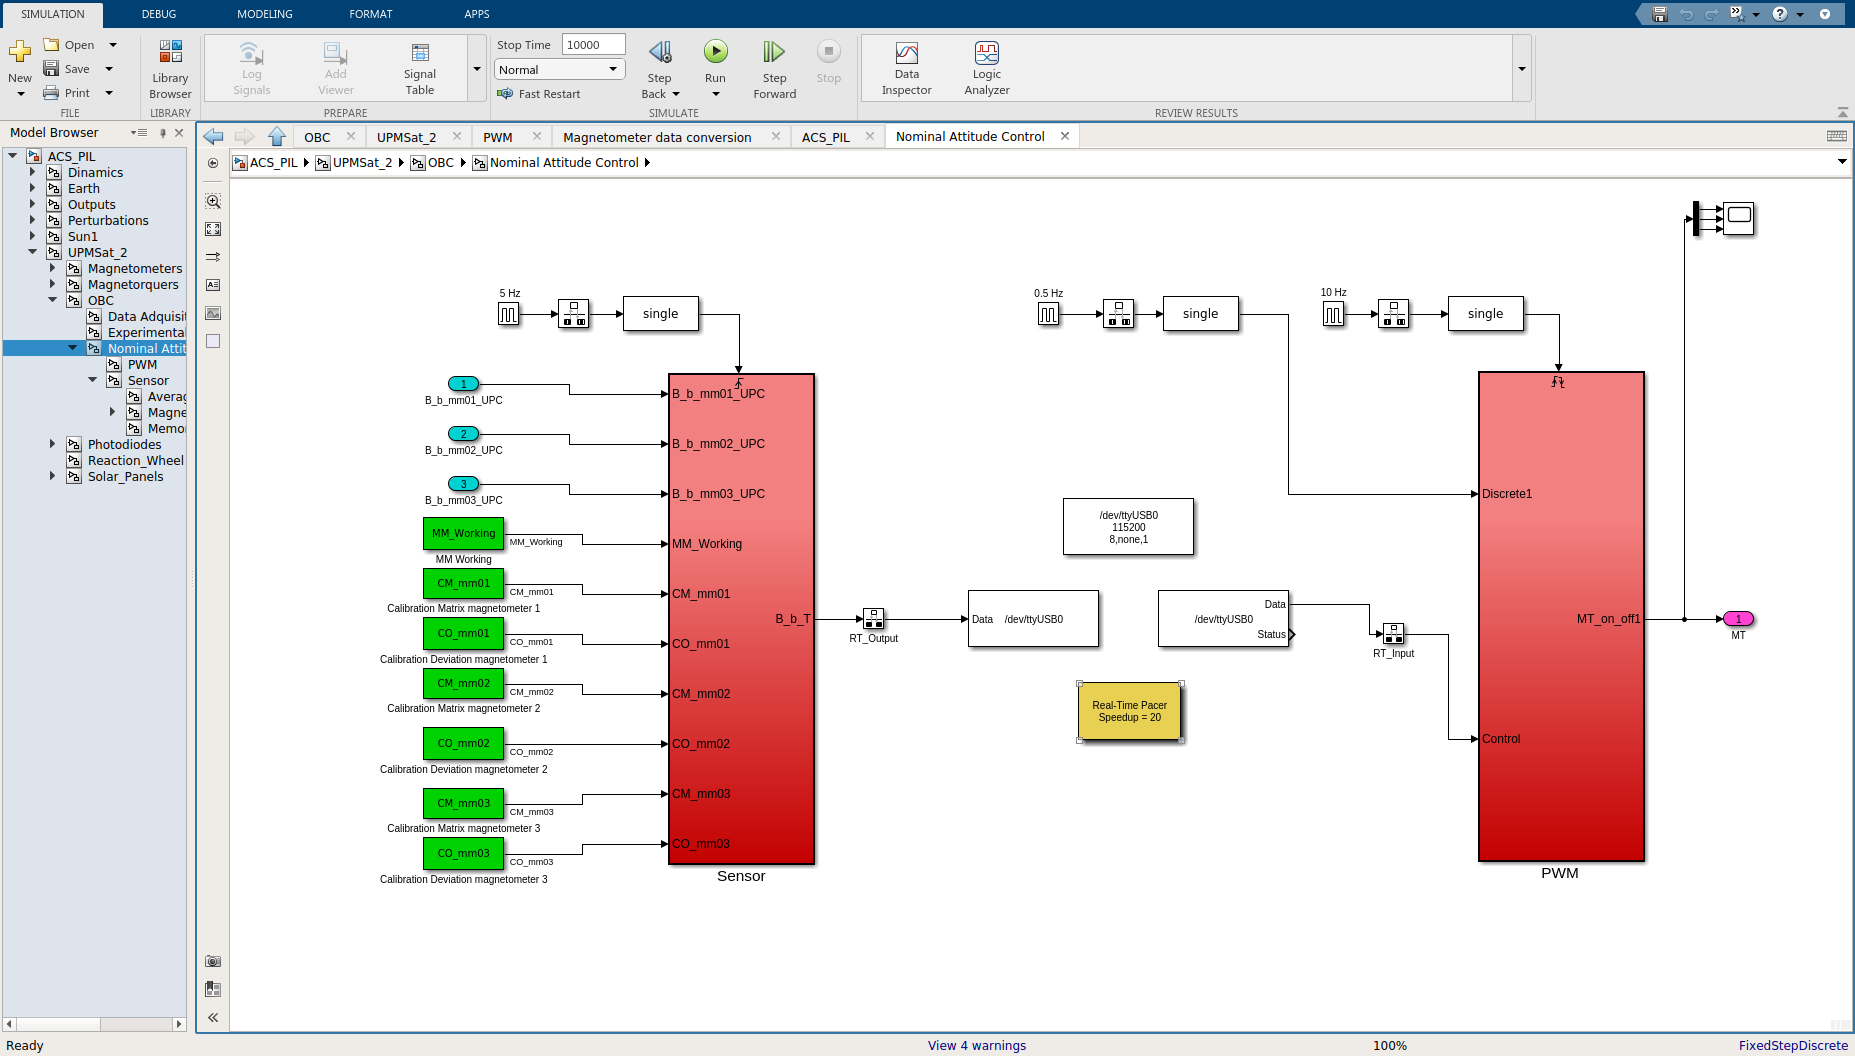
\includegraphics[width=\textwidth,keepaspectratio]{nac-pil.png}}
            \caption{Nominal attitude control for PIL.}
            \label{fig:nac-pil}
\end{figure}

Additional rate transition blocks has been added for a proper communication and a {\tt Real-Time Pacer} block has been also added to set the simulation speed\footnote{In a real case, an speedup equal to 1 should be used but it is to slow.}.

Start the simulation and verify angular velocity stabilization. Now ADC runs and red LED is toggled. 

\section{Make changes to the simulation.}

\begin{itemize}
\item Default parameters for control blocks can be changed in Ada source file {\tt ACS-parameters.ads}.
\begin{itemize}
\item {\tt Default\_omega} is the consigned angular velocity.
\item {\tt Default\_MT\_Working} contains the operational magneto-torques.
\end{itemize}

In UPMSat-2 many parameters can be changed by TC.
\item The initial angular velocity can be changed in Simulink source file {\tt initialization.m}.
\begin{itemize}
\item {\tt omega\_BI\_B0 = [0.1;-0.1;-0.1];}
\end{itemize}
\end{itemize}

\setcounter{chapter}{8}
\setcounter{section}{0}
\setcounter{figure}{0}
\setcounter{table}{0}
\renewcommand{\chaptername}{Final project}
\chapter*{Final project \\\vspace{7mm} OBDH system}\label{ch:obdh}
\addcontentsline{toc}{chapter}{OBDH system}
\markboth{FINAL PROJECT. OBDH SYSTEM}{FINAL PROJECT. OBDH SYSTEM}

The final version of the housekeeping program is a full OBDH system, including an additional sensor readings and the reception and interpretation of elementary telecommands from the ground station.

The ground station is implemented by a separate program running on the host PC platform. The radio connection between the OBDH software running on the OBC board and the ground station running on the host PC is simulated by a serial cable connection, as in assignments~\ref{ch:Assignment5} and~\ref{ch:Assignment6}.

\section{Software architecture and functional overview}

The software architecture is shown on figure~\ref{fig:obdh}. The system consists of four subsystems, very much like the ones found in a real on-board satellite system.

\begin{figure}[h]
            \centering{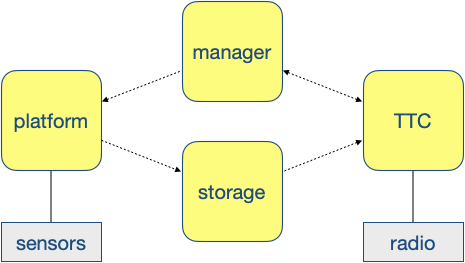
\includegraphics[width=.6\textwidth,keepaspectratio]{obdh.png}}
            \caption{OBDH system architecture.}
            \label{fig:obdh}
\end{figure}

\begin{itemize}
\item The {\tt platform} subsystem performs housekeeping functions on the satellite platform. It is expanded from the housekeeping component developed in the previous laboratory assignments in order to include an additional sensor. The list of variables that are monitored is now:
\begin{itemize}
\item OBC\_T : OBC temperature
\item OBC\_V : OBC voltage
\end{itemize}
The state of the platform is the set of values measured at a particular time, with a timestamp indicating the time at which they have been acquired. Mission time, a monotonic seconds count from the system start time, is used to this purpose.
\item The {\tt storage} subsystem keeps trace of the last N state values measured by the platform subsystem, where N is a configurable system parameter.
\item The {\tt TTC} system is in charge of all communications with the ground station. Its functionality includes:
\begin{itemize}
\item {\tt Telemetry} (TM) messages transmitted to ground, which may be of the following kinds:
\begin{itemize}
\item {\tt Basic} telemetry (Hello) messages, including the last measured values from all the sensors. These messages are periodically transmitted when the system is in idle mode (see below).
\item {\tt Housekeeping} messages include a more complete record with the last N stored values of the state. These messages are transmitted in response to a telecommand.
\item {\tt Mode} messages indicating the current operating mode of the system are transmitted after every mode change (see below).
\item {\tt Error} messages are occasionally sent to indicate some kinds of errors.
\end{itemize}
\item {\tt Telecommands} (TC) are messages received from ground, and can be of the following kinds:
\begin{itemize}
\item {\tt Open\_Link} messages are sent from the ground station in order to start a coverage period (see below).
\item {\tt Request\_HK} telecommands are used to request the OBDH system to send a housekeeping telemetry message.
\item {\tt Close\_Link} telecommands are sent by the ground station in order to close a coverage period and return to the idle mode (see below).
\item An {\tt error} TC value is signalled by the TTC subsystem when a message received from ground cannot be properly decoded as a valid TC.
\end{itemize}
\end{itemize}
\item The {\tt manager} subsystem carries out functions related to the operating mode of the system and the execution of telecommands. In this simplified OBDH system only two modes of operation are defined, related to the (simulated) visibility of the satellite from the ground station.
\begin{itemize}
\item {\tt Idle}. The system is this mode when the satellite is not visible from the ground station.
\item {\tt Coverage}. The system is in coverage mode when the satellite is visible from the ground station.
\end{itemize}
Mode changes are started from the TTC subsystem, according to the following protocol:
\item When in {\tt idle} mode, the OBDH system periodically transmits basic TM messages, and listens to telecommands from ground. When an open\_link TC is received, it requests the manager to switch to the coverage mode. No other kinds of telecommands are accepted in this mode.
\item When in {\tt coverage} mode, basic telemetry is not transmitted, and the TTC subsystem listens to telecommands from the ground station. The system switches back to idle mode when a close link TC is received or, alternatively, a maximum coverage time span has passed.
\end{itemize}

\section{System design}
The task structure of the system that has been designed in order to provide the above functionality is shown on figure~\ref{fig:obdh-task}.
\begin{figure}[h]
            \centering{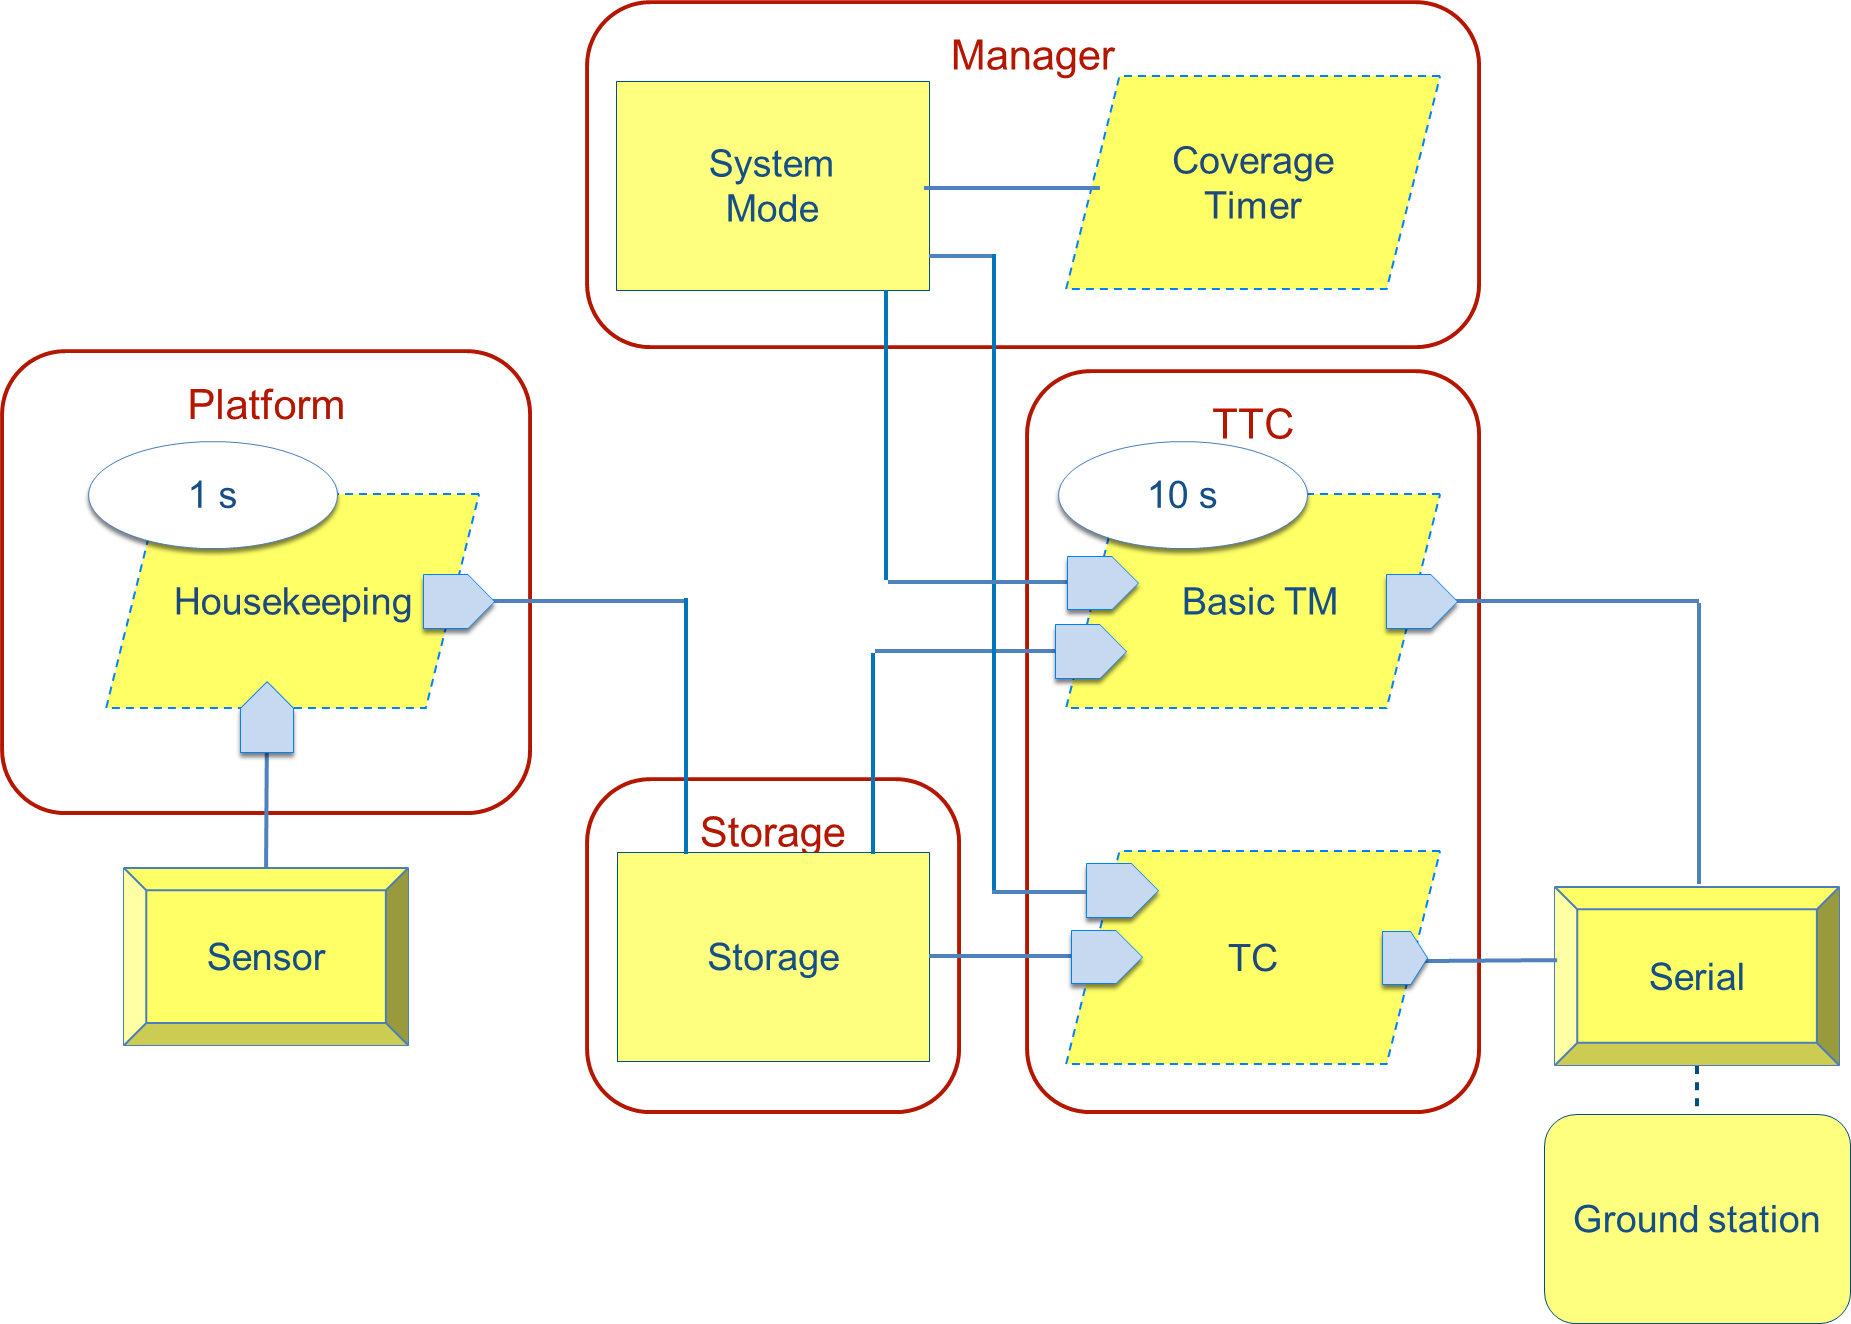
\includegraphics[width=\textwidth,keepaspectratio]{obdh-task.png}}
            \caption{OBDH system task structure.}
            \label{fig:obdh-task}
\end{figure}

\section{Real-time requirements}

The following real-time requirements are specified for the system:
\begin{itemize}
\item The {\tt Housekeeping} task executes with a period of 1 s and has a deadline of 100 ms.
\item The {\tt Basic\_TM} task executes with a period of 10 s and has a deadline of 500 ms.
\item The {\tt TC} task is sporadic, and is executed upon reception of a telecommand. The minimum separation of the event is 2 s, and the deadline is 1 s.
\item The {\tt Coverage\_Timer} task is sporadic with a minimum separation of 60 s and a deadline of 1 s.
\end{itemize}
Priorities are assigned in deadline-monotonic order, as shown in table~\ref{tb:obdh-requeriments}. The {\tt Buffer} protected object, which is part of the {\tt Storage} implementation, is accessed by the {\tt Housekeeping}, {\tt Basic\_TM} and {\tt TC} tasks, and thus has a ceiling priority equal to the priority of the {\tt Housekeeping} task.

\begin{table}[htb]
\begin{center}
\begin{tabular}{|l|r|r|r|} \hline
Task & Period & Deadline & Priority\\ \hline
Housekeeping & 1.0 & 1.0 & 20 \\
Coverage\_Timer & 60.0 & 1.0 & 15 \\
Basic\_TM & 10.0 & 0.5 & 12 \\
TC & 1.0 & 1.0 & 10 \\
Storage buffer & - & - & 20 \\ \hline
\end{tabular}
\caption{OBDH real-time requeriments.}
\label{tb:obdh-requeriments}
\end{center}
\end{table}

\section{Download the code and study the implementation}


The implementation code, as initially provided to the students, can be downloaded from \url{https://github.com/STR-UPM/OBDH\_LABS}. Click on {\tt Clone} or {\tt download}, download a zip archive, unzip and move to your work directory. The code for the OBDH system is in the PROJECT/OBDH folder.

The implementation code reflects the task structure in figure~\ref{fig:obdh-task}.

\section{Compile and run.}

Open GPS and do the following:
\begin{enumerate}
\item Select {\tt Open} project on the welcome window. Navigate to the PROJECT/OBDH directory and open the {\tt obdh.gpr} project file.
\item Build the executable and load it into the board by clicking on the \hbox{
\includegraphics[width=1.5em]{buildandload.png}} symbol in the tool bar (or select {\tt Build} > {\tt Bareboard} > {\tt Flash to board} on the top menu).

The program will be compiled, and the executable will be loaded into the board flash memory. After that, the program starts to run on the board (check the blinking LEDs).
\item Connect the serial cable to a USB port on the host computer, if not already done, following the instructions in section~\ref{sc:serial} of this manual.

\item Identify the serial port name on the host computer and launch the remote terminal application as explained in section~\ref{sc:term}.The output shows all telemetry messages received from the board, including basic housekeeping
in idle mode and responses to telecommands (figure~\ref{fig:obdh-output}).
\end{enumerate}

\begin{figure}[h]
            \centering{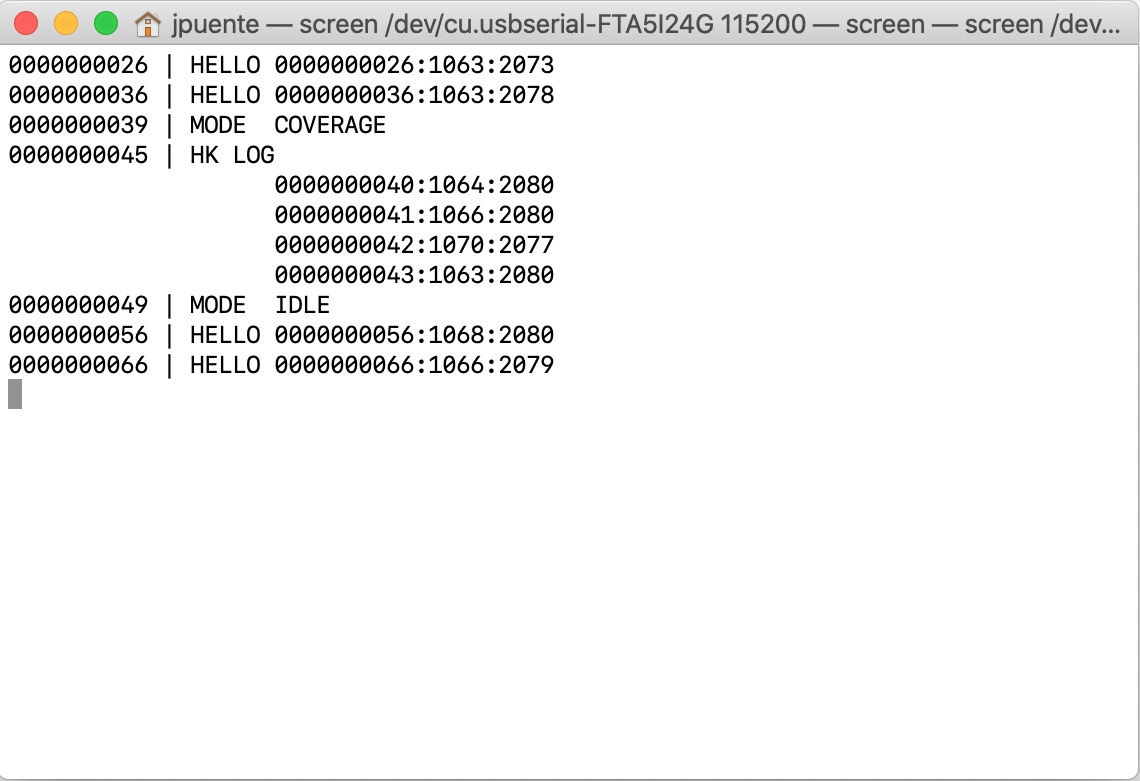
\includegraphics[width=0.6\textwidth,keepaspectratio]{obdh-output.png}}
            \caption{Sample telemetry messages received at the host terminal.}
            \label{fig:obdh-output}
\end{figure}

\section{Ground station}

The appearance of the output can be improved by using dedicated software. A simple example is the python script {\tt gs.py} located in PROJECT/GS directory. In order to use it, do the following:
\begin{enumerate}
\item Install Python in your system, if not already installed.
\item Install the {\tt pip} package manager if not already installed
\item Install the {\tt pySerial} module:
\begin{verbatim}
python -m pip install pyserial
\end{verbatim}
\item Edit the file {\tt gs.py} and set the serial port name on the host computer :
\begin{verbatim}
serial_port = 'COM4'
\end{verbatim}

\item Run the script from a terminal window, with the board connected to the host PC:
\begin{verbatim}
python gs.py
\end{verbatim}
\end{enumerate}
A sample of the telemetry messages received at the ground station is shown in figure~\ref{fig:gs-output}. The command ``exit'' terminates the execution of the ground station script.

\begin{figure}[h]
            \centering{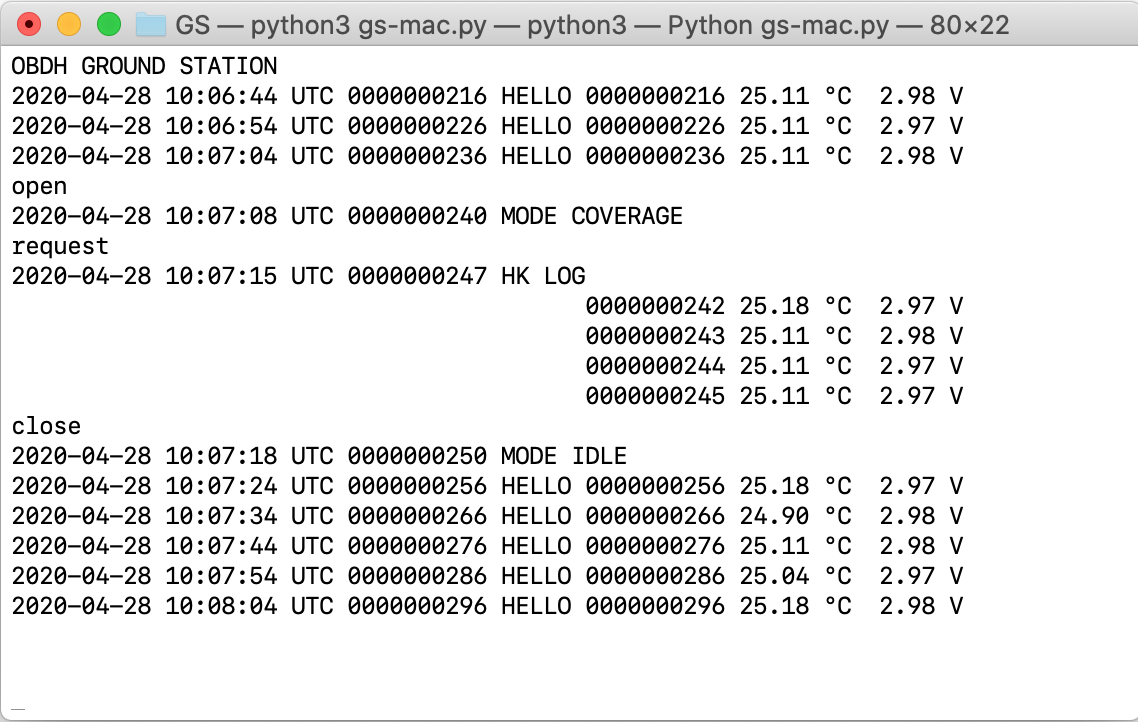
\includegraphics[width=0.6\textwidth,keepaspectratio]{gs-output.png}}
            \caption{Sample telemetry messages received at the GS script.}
            \label{fig:gs-output}
\end{figure}


%----------------------------------------------------------------------
%\cleardoublepage
%%\addcontentsline{toc}{section}{\protect\textbf{Appendices}}
%\appendix
%%\begin{appendices}
%% $Id: licence.tex,v 1.1.1.1 2001/11/02 16:06:27 ork Exp $
%---------------------------------------------------------------------------
\chapter{GNU General Public License}
\label{ap:licence}

\noindent
Version 2, June 1991

\noindent
\begin{raggedright}
Copyright \copyright\  1989, 1991 Free Software Foundation, Inc.\\
59 Temple Place - Suite 330, Boston, MA  02111-1307, USA.
\end{raggedright}

\vspace{\baselineskip}\noindent
Everyone is permitted to copy and distribute verbatim copies
of this license document, but changing it is not allowed.


\section*{Preamble}
  The licenses for most software are designed to take away your
freedom to share and change it.  By contrast, the GNU General Public
License is intended to guarantee your freedom to share and change free
software--to make sure the software is free for all its users.  This
General Public License applies to most of the Free Software
Foundation's software and to any other program whose authors commit to
using it.  (Some other Free Software Foundation software is covered by
the GNU Library General Public License instead.)  You can apply it to
your programs, too.

  When we speak of free software, we are referring to freedom, not
price.  Our General Public Licenses are designed to make sure that you
have the freedom to distribute copies of free software (and charge for
this service if you wish), that you receive source code or can get it
if you want it, that you can change the software or use pieces of it
in new free programs; and that you know you can do these things.

  To protect your rights, we need to make restrictions that forbid
anyone to deny you these rights or to ask you to surrender the rights.
These restrictions translate to certain responsibilities for you if you
distribute copies of the software, or if you modify it.

  For example, if you distribute copies of such a program, whether
gratis or for a fee, you must give the recipients all the rights that
you have.  You must make sure that they, too, receive or can get the
source code.  And you must show them these terms so they know their
rights.

  We protect your rights with two steps: (1) copyright the software, and
(2) offer you this license which gives you legal permission to copy,
distribute and/or modify the software.

  Also, for each author's protection and ours, we want to make certain
that everyone understands that there is no warranty for this free
software.  If the software is modified by someone else and passed on, we
want its recipients to know that what they have is not the original, so
that any problems introduced by others will not reflect on the original
authors' reputations.

  Finally, any free program is threatened constantly by software
patents.  We wish to avoid the danger that redistributors of a free
program will individually obtain patent licenses, in effect making the
program proprietary.  To prevent this, we have made it clear that any
patent must be licensed for everyone's free use or not licensed at all.

  The precise terms and conditions for copying, distribution and
modification follow.

\section*{Terms and conditions for copying, distribution and modification}

\begin{enumerate}
\setcounter{enumi}{-1}

\item
This License applies to any program or other work which contains
a notice placed by the copyright holder saying it may be distributed
under the terms of this General Public License.  The "Program", below,
refers to any such program or work, and a "work based on the Program"
means either the Program or any derivative work under copyright law:
that is to say, a work containing the Program or a portion of it,
either verbatim or with modifications and/or translated into another
language.  (Hereinafter, translation is included without limitation in
the term "modification".)  Each licensee is addressed as "you".

Activities other than copying, distribution and modification are not
covered by this License; they are outside its scope.  The act of
running the Program is not restricted, and the output from the Program
is covered only if its contents constitute a work based on the
Program (independent of having been made by running the Program).
Whether that is true depends on what the Program does.

\item
 You may copy and distribute verbatim copies of the Program's
source code as you receive it, in any medium, provided that you
conspicuously and appropriately publish on each copy an appropriate
copyright notice and disclaimer of warranty; keep intact all the
notices that refer to this License and to the absence of any warranty;
and give any other recipients of the Program a copy of this License
along with the Program.

You may charge a fee for the physical act of transferring a copy, and
you may at your option offer warranty protection in exchange for a fee.

\item
 You may modify your copy or copies of the Program or any portion
of it, thus forming a work based on the Program, and copy and
distribute such modifications or work under the terms of Section 1
above, provided that you also meet all of these conditions:

\begin{enumerate}
\item
     You must cause the modified files to carry prominent notices
     stating that you changed the files and the date of any change.

\item
     You must cause any work that you distribute or publish, that in
     whole or in part contains or is derived from the Program or any
     part thereof, to be licensed as a whole at no charge to all third
     parties under the terms of this License.

\item
     If the modified program normally reads commands interactively
     when run, you must cause it, when started running for such
     interactive use in the most ordinary way, to print or display an

     announcement including an appropriate copyright notice and a
     notice that there is no warranty (or else, saying that you provide
     a warranty) and that users may redistribute the program under
     these conditions, and telling the user how to view a copy of this
     License.  (Exception: if the Program itself is interactive but
     does not normally print such an announcement, your work based on
     the Program is not required to print an announcement.)
\end{enumerate}

These requirements apply to the modified work as a whole.  If
identifiable sections of that work are not derived from the Program,
and can be reasonably considered independent and separate works in
themselves, then this License, and its terms, do not apply to those
sections when you distribute them as separate works.  But when you
distribute the same sections as part of a whole which is a work based
on the Program, the distribution of the whole must be on the terms of
this License, whose permissions for other licensees extend to the
entire whole, and thus to each and every part regardless of who wrote it.

Thus, it is not the intent of this section to claim rights or contest
your rights to work written entirely by you; rather, the intent is to
exercise the right to control the distribution of derivative or
collective works based on the Program.

In addition, mere aggregation of another work not based on the Program
with the Program (or with a work based on the Program) on a volume of
a storage or distribution medium does not bring the other work under
the scope of this License.

\item
 You may copy and distribute the Program (or a work based on it,
under Section 2) in object code or executable form under the terms of
Sections 1 and 2 above provided that you also do one of the following:

\begin{enumerate}
\item
     Accompany it with the complete corresponding machine-readable
     source code, which must be distributed under the terms of Sections
     1 and 2 above on a medium customarily used for software interchange; or,

\item
     Accompany it with a written offer, valid for at least three
     years, to give any third party, for a charge no more than your
     cost of physically performing source distribution, a complete
     machine-readable copy of the corresponding source code, to be
     distributed under the terms of Sections 1 and 2 above on a medium
     customarily used for software interchange; or,

\item
     Accompany it with the information you received as to the offer
     to distribute corresponding source code.  (This alternative is
     allowed only for noncommercial distribution and only if you
     received the program in object code or executable form with such
     an offer, in accord with Subsection b above.)
\end{enumerate}

The source code for a work means the preferred form of the work for
making modifications to it.  For an executable work, complete source
code means all the source code for all modules it contains, plus any
associated interface definition files, plus the scripts used to
control compilation and installation of the executable.  However, as a
special exception, the source code distributed need not include
anything that is normally distributed (in either source or binary
form) with the major components (compiler, kernel, and so on) of the
operating system on which the executable runs, unless that component
itself accompanies the executable.

If distribution of executable or object code is made by offering
access to copy from a designated place, then offering equivalent
access to copy the source code from the same place counts as
distribution of the source code, even though third parties are not
compelled to copy the source along with the object code.

\item
 You may not copy, modify, sublicense, or distribute the Program
except as expressly provided under this License.  Any attempt
otherwise to copy, modify, sublicense or distribute the Program is
void, and will automatically terminate your rights under this License.
However, parties who have received copies, or rights, from you under
this License will not have their licenses terminated so long as such
parties remain in full compliance.

\item
 You are not required to accept this License, since you have not
signed it.  However, nothing else grants you permission to modify or
distribute the Program or its derivative works.  These actions are
prohibited by law if you do not accept this License.  Therefore, by
modifying or distributing the Program (or any work based on the
Program), you indicate your acceptance of this License to do so, and
all its terms and conditions for copying, distributing or modifying
the Program or works based on it.

\item
 Each time you redistribute the Program (or any work based on the
Program), the recipient automatically receives a license from the
original licensor to copy, distribute or modify the Program subject to
these terms and conditions.  You may not impose any further
restrictions on the recipients' exercise of the rights granted herein.
You are not responsible for enforcing compliance by third parties to
this License.

\item
 If, as a consequence of a court judgment or allegation of patent
infringement or for any other reason (not limited to patent issues),
conditions are imposed on you (whether by court order, agreement or
otherwise) that contradict the conditions of this License, they do not
excuse you from the conditions of this License.  If you cannot
distribute so as to satisfy simultaneously your obligations under this
License and any other pertinent obligations, then as a consequence you
may not distribute the Program at all.  For example, if a patent
license would not permit royalty-free redistribution of the Program by
all those who receive copies directly or indirectly through you, then
the only way you could satisfy both it and this License would be to
refrain entirely from distribution of the Program.

If any portion of this section is held invalid or unenforceable under
any particular circumstance, the balance of the section is intended to
apply and the section as a whole is intended to apply in other
circumstances.

It is not the purpose of this section to induce you to infringe any
patents or other property right claims or to contest validity of any
such claims; this section has the sole purpose of protecting the
integrity of the free software distribution system, which is
implemented by public license practices.  Many people have made
generous contributions to the wide range of software distributed
through that system in reliance on consistent application of that
system; it is up to the author/donor to decide if he or she is willing
to distribute software through any other system and a licensee cannot
impose that choice.

This section is intended to make thoroughly clear what is believed to
be a consequence of the rest of this License.

\item
 If the distribution and/or use of the Program is restricted in
certain countries either by patents or by copyrighted interfaces, the
original copyright holder who places the Program under this License
may add an explicit geographical distribution limitation excluding
those countries, so that distribution is permitted only in or among
countries not thus excluded.  In such case, this License incorporates
the limitation as if written in the body of this License.


\item
 The Free Software Foundation may publish revised and/or new versions
of the General Public License from time to time.  Such new versions will
be similar in spirit to the present version, but may differ in detail to
address new problems or concerns.

Each version is given a distinguishing version number.  If the Program
specifies a version number of this License which applies to it and "any
later version", you have the option of following the terms and conditions
either of that version or of any later version published by the Free
Software Foundation.  If the Program does not specify a version number of
this License, you may choose any version ever published by the Free Software
Foundation.


\item
 If you wish to incorporate parts of the Program into other free
programs whose distribution conditions are different, write to the author
to ask for permission.  For software which is copyrighted by the Free
Software Foundation, write to the Free Software Foundation; we sometimes
make exceptions for this.  Our decision will be guided by the two goals
of preserving the free status of all derivatives of our free software and
of promoting the sharing and reuse of software generally.

\subsection*{NO WARRANTY}

\item
 BECAUSE THE PROGRAM IS LICENSED FREE OF CHARGE, THERE IS NO WARRANTY
FOR THE PROGRAM, TO THE EXTENT PERMITTED BY APPLICABLE LAW.  EXCEPT WHEN
OTHERWISE STATED IN WRITING THE COPYRIGHT HOLDERS AND/OR OTHER PARTIES
PROVIDE THE PROGRAM "AS IS" WITHOUT WARRANTY OF ANY KIND, EITHER EXPRESSED
OR IMPLIED, INCLUDING, BUT NOT LIMITED TO, THE IMPLIED WARRANTIES OF
MERCHANTABILITY AND FITNESS FOR A PARTICULAR PURPOSE.  THE ENTIRE RISK AS
TO THE QUALITY AND PERFORMANCE OF THE PROGRAM IS WITH YOU.  SHOULD THE
PROGRAM PROVE DEFECTIVE, YOU ASSUME THE COST OF ALL NECESSARY SERVICING,
REPAIR OR CORRECTION.

\item
 IN NO EVENT UNLESS REQUIRED BY APPLICABLE LAW OR AGREED TO IN WRITING
WILL ANY COPYRIGHT HOLDER, OR ANY OTHER PARTY WHO MAY MODIFY AND/OR
REDISTRIBUTE THE PROGRAM AS PERMITTED ABOVE, BE LIABLE TO YOU FOR DAMAGES,
INCLUDING ANY GENERAL, SPECIAL, INCIDENTAL OR CONSEQUENTIAL DAMAGES ARISING
OUT OF THE USE OR INABILITY TO USE THE PROGRAM (INCLUDING BUT NOT LIMITED
TO LOSS OF DATA OR DATA BEING RENDERED INACCURATE OR LOSSES SUSTAINED BY
YOU OR THIRD PARTIES OR A FAILURE OF THE PROGRAM TO OPERATE WITH ANY OTHER
PROGRAMS), EVEN IF SUCH HOLDER OR OTHER PARTY HAS BEEN ADVISED OF THE
POSSIBILITY OF SUCH DAMAGES.
\end{enumerate}


\section*{End of terms and conditions}

\newpage
\section*{How to Apply These Terms to Your New Programs}

  If you develop a new program, and you want it to be of the greatest
possible use to the public, the best way to achieve this is to make it
free software which everyone can redistribute and change under these terms.

  To do so, attach the following notices to the program.  It is safest
to attach them to the start of each source file to most effectively
convey the exclusion of warranty; and each file should have at least
the "copyright" line and a pointer to where the full notice is found.

\begin{quotation}
\begin{alltt}\scriptsize\noindent
\emph{one line to give the program's name and an idea of what it does.}
Copyright \copyright\  \emph{yyyy}  \emph{name of author}

This program is free software; you can redistribute it and/or
modify it under the terms of the GNU General Public License
as published by the Free Software Foundation; either version 2
of the License, or (at your option) any later version.

This program is distributed in the hope that it will be useful,
but WITHOUT ANY WARRANTY; without even the implied warranty of
MERCHANTABILITY or FITNESS FOR A PARTICULAR PURPOSE.  See the
GNU General Public License for more details.

You should have received a copy of the GNU General Public License
along with this program; if not, write to the Free Software
Foundation, Inc., 59 Temple Place - Suite 330, Boston, MA  02111-1307, USA.
\end{alltt}
\end{quotation}


Also add information on how to contact you by electronic and paper mail.

If the program is interactive, make it output a short notice like this
when it starts in an interactive mode:

\begin{quotation}
\begin{alltt}\scriptsize\noindent
Gnomovision version 69, Copyright (C) \emph{year} \emph{name of author}
Gnomovision comes with ABSOLUTELY NO WARRANTY; for details
type `show w'.  This is free software, and you are welcome
to redistribute it under certain conditions; type `show c'
for details.
\end{alltt}
\end{quotation}

The hypothetical commands \texttt{`show w'} and \texttt{`show c'} should show
the appropriate parts of the General Public License.  Of course, the
commands you use may be called something other than \texttt{`show w'} and
\texttt{`show c'}; they could even be mouse-clicks or menu items--whatever
suits your program.

You should also get your employer (if you work as a programmer) or your
school, if any, to sign a "copyright disclaimer" for the program, if
necessary.  Here is a sample; alter the names:

\begin{quotation}
\begin{alltt}\scriptsize\noindent
Yoyodyne, Inc., hereby disclaims all copyright
interest in the program `Gnomovision'
(which makes passes at compilers) written
by James Hacker.
\emph{signature of Ty Coon}, 1 April 1989
Ty Coon, President of Vice
\end{alltt}
\end{quotation}

This General Public License does not permit incorporating your program into
proprietary programs.  If your program is a subroutine library, you may
consider it more useful to permit linking proprietary applications with the
library.  If this is what you want to do, use the GNU Library General
Public License instead of this License.

%%\end{appendices}
%======================= back matter ===================================
%\addcontentsline{toc}{chapter}{\numberline{}Bibliography}
%\bibliography{realtime,anser}
%\cleardoublepage
\end{document}

